\chapter{Electronic Circuits}

\section*{Objectives}

\begin{enumerate}
\item To study the response of an RC circuit as a low-pass Filter and a high-pass Filter.
\item To study the response of an LCR circuit in different configurations.
\end{enumerate}


\section*{Introduction}

When a potential difference is applied across a conductor, it causes a flow of electrons known as a \textsl{current}. An ideal conductor will be able to sustain such a current indefinitely without losing any energy. However, in realistic conductors, the amount of current that can flow is limited by a material property of the conductor known as the ``resistivity''. To model such realistic systems, in our simplified circuits we consider an electronic component known as a \textsl{resistor}. We imagine an ideal resistor constructed as shown in Figure~(\ref{fig:electronics-components}): two perfectly conducting wires attach to two ends of a ``bar'' of resistive material. In such an ideal resistor, it then follows that the applied voltage $V$ and the produced current $I$ are proportional to each other through a constant of proportionality known as the ``Resistance'' of the resistor $R$. Thus, we get what is commonly known as Ohm's law,
\begin{equation}
    V = I R.
    \label{eqn:ohms-law}
\end{equation}

In more advanced courses, you will see that this linear relationship between the current and the voltage is only approximate for real conducting materials. However, this approximation is more than sufficient for our purposes.


\begin{figure}[!htb]
    \centering
    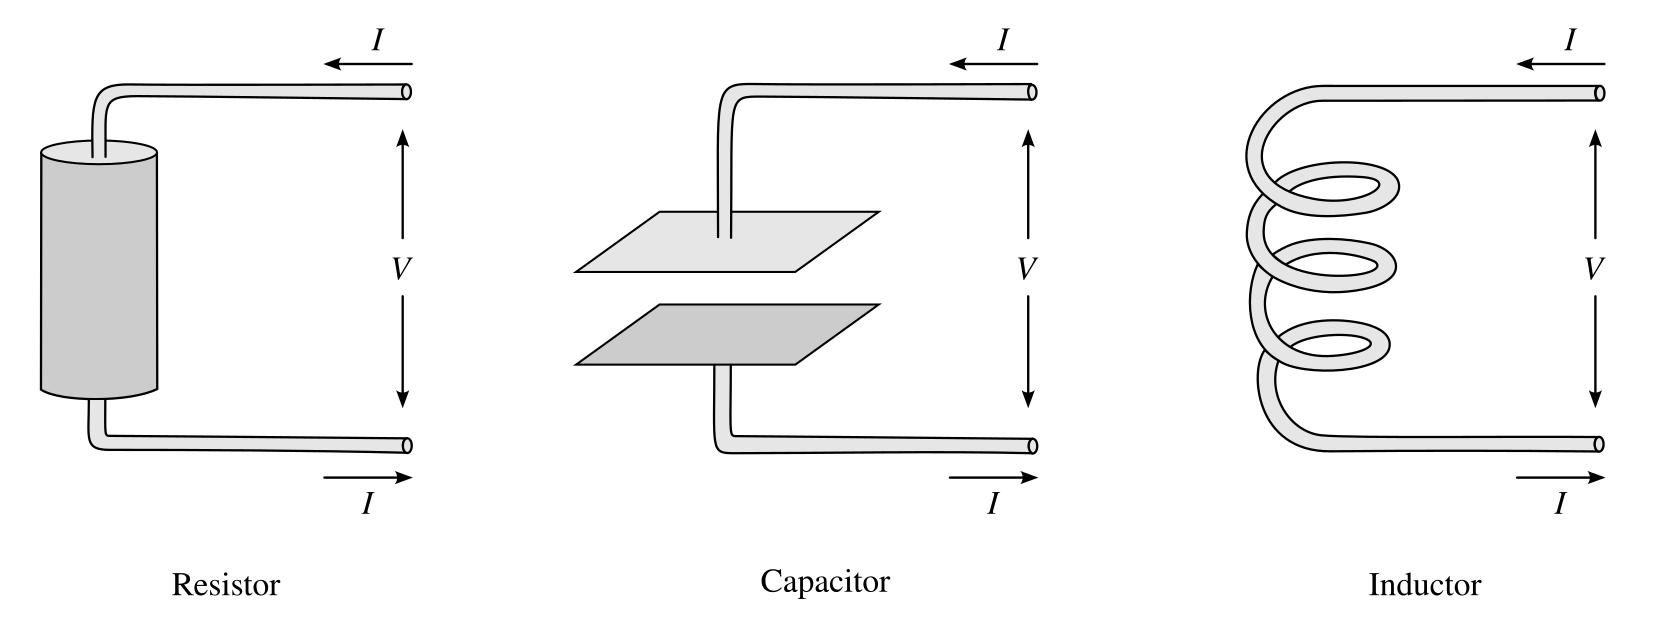
\includegraphics[width=\textwidth]{figs/electronics-circuits/electronics-components.png}
    \caption{Three passive circuit components. Resistors are conductors  }
    \label{fig:electronics-components}
\end{figure}



You should all be quite familiar with resistances by now. Figure~(\ref{fig:electronics-components}) also shows two other electronics components with which you are perhaps less familiar. The first of these is a ``capacitor''. As shown in the figure, a capacitor consists of two perfectly conducting wires attached independently to two perfectly conducting plates. When a constant voltage is applied across such a system, it causes a flow of current. However, since the two plates are not in contact with each other, the current simply leads to a build-up of charge on each of the capacitor's plates. The net charge in the system being constant implies that the upper plate accumulates a charge of $+Q$, while the lower accumulates a charge of $-Q$. It can be shown that the potential difference between the plates $V$ is proportional to this charge, and that 
\begin{equation}
    V = \frac{Q}{C},
    \label{eqn:def-cap}
\end{equation}

where $C$ is a constant for a capacitor, known as its ``capacitance''.

The last component is the inductor. An inductor is constructed by winding many turns of a perfectly conducting wire in the form of a coil, and bringing the two ends out to terminals at some distance from the coil. When a voltage $V$ is applied across such a system, it causes a current $I$ which produces a magnetic field as it flows through the loops. In an ideal inductor, we assume that the magnetic field remains contained within the coil. We further assume that in such an ideal system, the wire has no resistance, and that there is no build-up of charge on the surface of the wires. When a current passes through such a coil, a magnetic field proportional to the current is built up inside it. If the current changes as a function of time, this magnetic field also changes. From Lenz's law, you should recall that such a changing magnetic field induces an electromotive force which translates to an induced voltage. The voltage generated in this way can be shown to be 
\begin{equation}
    V = L \dv{I}{t},
    \label{eqn:def-ind}
\end{equation}

where $L$ is a constant for an inductor, known as its ``inductance''.

The way we have described the above components illustrates a general approach that we will take in analysing circuits: the properties of these components are described completely in terms of the currents and voltages that are measured at the \textsl{terminals}. This allows us -- provided certain simplifying assumptions are made -- to ignore the great complexities of the inner workings of these components.

In the description of the inductor given above, you should be able to see that it behaves differently depending on the type of current passed through the circuit. If a constant current flows through an inductor, it essentially behaves like an ideal conducting wire. However, if instead we provide a time-varying current, a potential drop will be observed across the inductor, by an amount proportional to its inductance $L$. Thus, we see that our circuit components need not behave in the same way when exposed to constant ``direct'' current (DC) or ``alternating'' current (AC).

In fact, it is much more general than this. As we shall see, certain circuit elements like inductors and capacitors exhibit a \textsl{frequency} response, meaning that they behave differently when different frequencies of AC are passed through them. This is precisely what you will be studying throughout this experiment.


\section*{Theory}

We will now motivate the basic responses of resistors, capacitors, and inductors to alternating current. Keep in mind that unless explicitly stated, we will be assuming that our circuit components are all \textsl{ideal}. In reality, this is of course an approximation, but one that is valid in our experimental conditions.

One of the consequences of assuming ideal components is that we will be dealing with \textsl{linear} systems. You will see such systems appear throughout your physics curriculum, which is why they are so important to study. As we shall see, the mathematics of our simple electrical systems maps perfectly onto the mathematics of simple mechanical systems, meaning that all of our electrical systems have mechanical analogues. 

Additionally, we will only be dealing with systems in which the voltages and currents varying sinusoidally. Such sinusoidally varying systems are characterised by an \textsl{amplitude} and a \textsl{phase}. In general, a voltage $V(t)$ that varies in this fashion can be expressed as 
\begin{equation}
    V(t) = V_0 \cos(\omega t + \varphi),
\end{equation}

where $V_0$ is its amplitude, $\omega$ its frequency, and $\varphi$ is its phase. However, such sinusoids are often slightly cumbersome to work with mathematically. However, it turns out that since we are working with linear systems, we can instead work with \textsl{complex} exponentials, which naturally allow us to characterise the amplitude and the phase with a single complex number. Thus, a time-varying voltage $V(t)$ can be written as 
\begin{equation}
    V(t) = \widetilde{V} e^{i\omega t} = V_0 e^{i\varphi} e^{i\omega t},
    \label{eqn:comp-exp}
\end{equation}

where $\widetilde{V}$ is a complex number independent of $t$, and the time-dependence is completely encapsulated in the complex exponential.

\begin{imp}
    It is, of course, understood that the actual time-varying voltage $V(t)$ is  given by the \textsl{real part} of the right-hand side of Equation~(\ref{eqn:comp-exp}). The voltages are clearly not actually complex numbers; however, the operations that we will perform on them will be linear operations that do not mix the real and imaginary parts. Additionally, it is much easier to work with complex exponentials when compared to real sinusoids. Therefore, if we remind ourselves that the quantities of interest are always the real parts of our variables, we can use the complex notation to get the same answers.
\end{imp}

Thus, all the time-varying quantities in our analyses will be taken to vary with the same frequency $\omega$, and therefore
\begin{equation}
    \begin{aligned}
        V(t) &= \widetilde{V} e^{i\omega t},\\
        I(t) &= \widetilde{I} e^{i \omega t}. 
    \end{aligned}
    \label{eqn:time-dep}
\end{equation}

Most of the time we will write our equations in terms of $V$ and $I$, with the implicit understanding that the time-dependence is given by Equation~(\ref{eqn:time-dep}).

\begin{imp}
    Note that our complex notation will only work so long as the operations that we are performing are \textsl{linear}. In particular, if we were to compute the power $P(t) = V(t) I(t)$ and were to naively multiply the two terms in Equation~(\ref{eqn:time-dep}) and take the resulting real part, we wouldn't get the right answer. For such non-linear terms, one should either first extract the real part and then multiply them together, or alternatively a new definition of products will need to be used. However, we will not be concerning ourselves with this right now.
\end{imp}



\subsection*{Responses to time-varying systems}

Given the above assumptions, we can now ask ourselves how our individual components will respond to time-varying signals. 

\begin{question}
    \textbf{Question:} Using Equations~(\ref{eqn:ohms-law})~--~(\ref{eqn:def-ind}), show that the ratio $z$ of the voltage to the current is given by
    \begin{equation}
        \begin{aligned}
            z_R &= \frac{V}{I} = R &&\text{for an ideal resistor}, \\[10pt]
            z_C &= \frac{V}{I} = \frac{1}{i\omega C} &&\text{for an ideal capacitor}, \\[10pt]
            z_L &= \frac{V}{I} = i \omega L &&\text{for an ideal inductor}.
        \end{aligned}
        \label{eqn:def-impedance}
    \end{equation}
    \textbf{Hint:} For the capacitor, take the derivative of Equation~(\ref{eqn:def-cap}).
\end{question}

There are many things to notice in Equation~(\ref{eqn:def-impedance}). Firstly, the voltage is always proportional to the current, with a coefficient of proportionality $z$ that is different for resistors, capacitors, and inductors. Secondly, this coefficient of proportionality is, in general, a complex number. And lastly, $z$ is also a function of the frequency $\omega$ in general. For a pure resistor, however, $z$ is simply the resistance. This leads us to the conclusion that $z$ is the \textsl{generalisation} of resistance to AC circuits, and is called the \textsl{impedance}.


\begin{figure}[!htb]
    \centering
    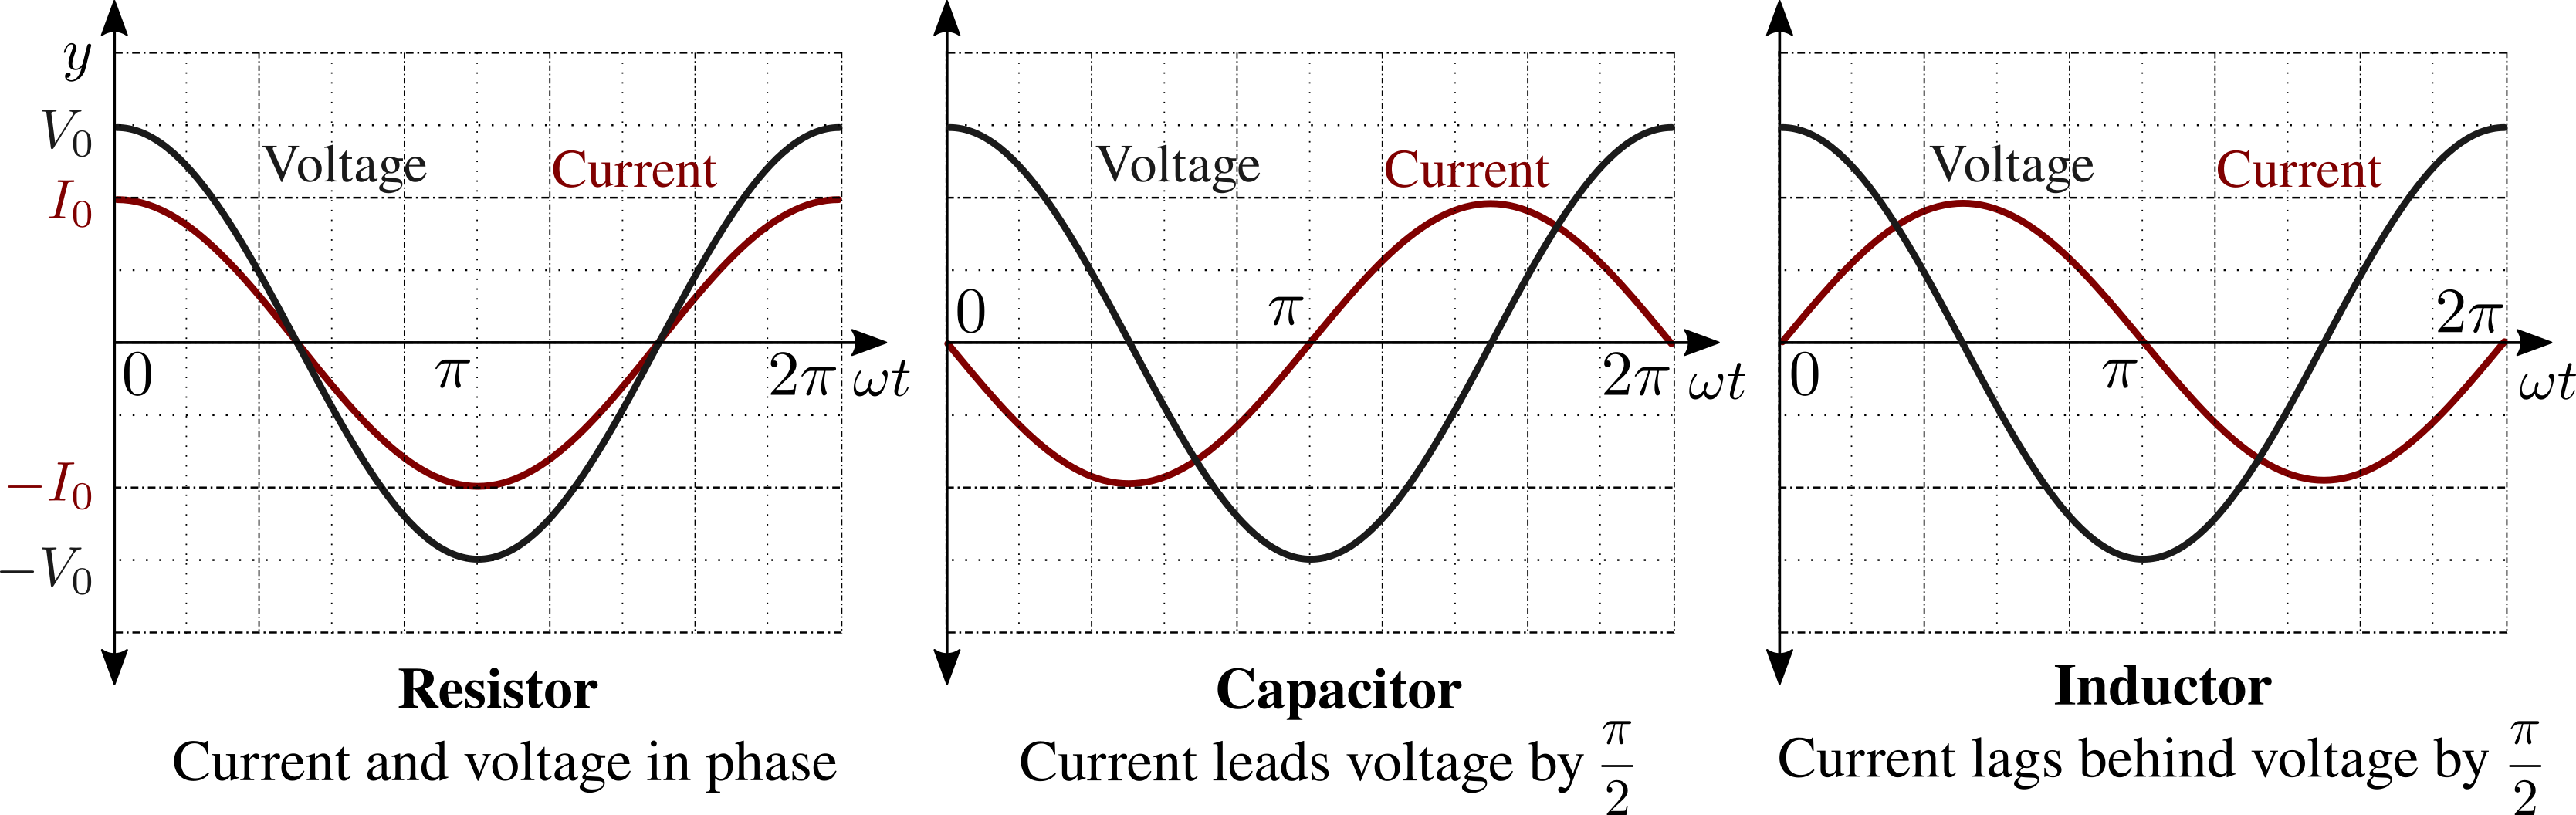
\includegraphics[width=\textwidth]{figs/electronics-circuits/electronics-components-phase-graphs.png}
    \caption{The components described above affect not only the amplitude of the current but also its phase with respect to the applied voltage. For a resistor, the current and voltage are in phase. For a capacitor, the current leads by a phase of $\pi/2$. For an inductor, the current lags by the same phase of $\pi/2$. In order to decide whether the current lags or leads, first ask yourself how much you need to move the current curve so that it is in phase with the voltage. If, for example, you need to move the curve rightward, this means that the current at an \textsl{earlier} time was at the same phase as the voltage at a \textsl{later} time. This implies that the current leads the voltage.  }
    \label{fig:phase-graphs}
\end{figure}



\begin{question}
    \textbf{Question:} Consider a simple time-varying voltage 
    \begin{equation}
        V(t) = V_0 e^{i\omega t},
    \end{equation}
    where $V_0$ is real. Show that the resulting (real) current in the case of each of the above components is given by
    \begin{equation}
        \begin{aligned}
            I_R &= \frac{V_0}{R} \cos(\omega t),\\[10pt]
            I_C &= - \omega C V_0 \sin(\omega t),\\[10pt]
            I_L &= + \frac{V_0}{L} \sin(\omega t).
        \end{aligned}
    \end{equation}

    \textbf{Question:} Use this to show that
    \vspace{-\parskip}
    \begin{enumerate}
    \itemsep0em
        \item In resistors, the current and voltage are in phase,
        \item In capacitors, the current leads the voltage by a phase of $\pi/2$,
        \item In inductors, the current lags behind the the voltage by a phase of $\pi/2$.  
    \end{enumerate}
\end{question}

\begin{imp}
    Often, purely imaginary quantities $z_C$ and $z_L$ are known as ``reactance'', to distinguish themselves from the resistance. There is some merit in this, since these two quantities change both the magnitude of the current, as well as its \textsl{phase}. Resistance, on the other hand, being purely real, only affects the magnitude of the current. However, in our analyses we will just use the general terms impedance for all types of $z$. This is shown graphically in Figure~(\ref{fig:phase-graphs})
\end{imp}



\subsection*{The RC circuit}

We will now try to combine two components -- a resistor and a capacitor -- in a simple circuit. Consider first a capacitor being charged by a DC power source. As the key in switched on, the power source establishes a potential difference across the plates of the capacitor and stores some charge on them. The amount of charge stored is given by the definition of the capacitance in Equation~(\ref{eqn:def-cap}).

If the switch is now disconnected, the capacitor would hold this charge indefinitely. However, if the capacitor is allowed to discharge through a resistor, a current is set up in the circuit which dissipates the energy stored in the capacitor. Using Kirchoff's voltage law to this closed loop, the voltage drop across the resistor ad capacitor should add up to the applied voltage.

\begin{question}
\paragraph{Question:} Using Ohm's Law ($V=IR$) and the definition of capacitance ($Q=CV$), show that this means that:
\begin{equation*}
    R \dv{Q}{t} + \frac{Q}{C} = V_0
\end{equation*}
where $Q(t)$ is the instantaneous charge on the capacitor.

\paragraph{Question:} Solve this (simple) first-order differential equation for the following initial conditions:
\begin{enumerate}
    \item \textbf{Discharging:} The capacitor is initially charged $Q(0) = Q_0$, and is allowed to discharge. (There is no voltage source in the circuit.) \hfill\textbf{Answer:} $Q(t) = Q_0\,\, e^{-t/RC}.$
    
    \item \textbf{Charging:} The capacitor is initially uncharged $Q(0) = 0$, and is allowed to charge from a voltage source $V_0$.
    \hfill\textbf{Answer:} $Q(t) = Q_0\,\, \left(1 - e^{-t/RC}\right).$
\end{enumerate}
\end{question}


An important result from the above analysis is that we can construct a quantity of dimension time, $\tau = RC$, which is the natural time scale of charging or discharging the capacitor through the resistor. This quantity is often called the \textsl{time-constant} of the $RC$ circuit.

\subsection*{The RC circuit as an integrator and a differentiator}

Despite its simplicity, the $RC$ circuit can be used to perform complex tasks. Let us now consider how such a circuit responds to an AC signal of frequency $\omega$. In this case, the input and output voltages of our system are 
\begin{equation}
        V_\text{in}(t) = \widetilde{V}_\text{in} e^{i\omega t} \quad \quad \text{and} \quad \quad V_\text{out}(t) = \widetilde{V}_\text{out} e^{i\omega t}.
\end{equation}

We now have two different time-scales in our problem: one time-scale is the ``natural'' time-scale of the $RC$ circuit ($\tau = RC$), and the other is the time-period associated with the AC signal of frequency $\omega$. 

\subsubsection*{The RC integrator}

Consider what happens when we take the output voltage across the capacitor at \textsl{high} frequency, meaning that we choose a frequency 
\begin{equation}
    \omega \gg \frac{1}{RC}.
\end{equation}

Over this short time-scale, the capacitor barely has time to charge, and therefore the voltage across it is very small. In other words, the input voltage is almost completely dropped over the resistor,
\begin{equation}
    V_\text{in} \approx V_R.
\end{equation}

\begin{question}
    \textbf{Question:} Show the above result in the following way: first show that the current in the circuit is given by
    \begin{equation}
        I = \dfrac{V_\text{in}}{R + \dfrac{1}{i\omega C}}.
        \label{eqn:RC-current}
    \end{equation}

    Next, using the fact that $\omega \gg 1/RC$, show that this just means that 
    \begin{equation}
        I(t) \approx \frac{V_\text{in} (t)}{R},
        \label{eqn:high-freq-current}
    \end{equation}
    which is simply Ohm's law that we saw in Equation~(\ref{eqn:ohms-law}).

    Thus argue that $V_\text{in} \approx V_R$, the potential drop across the resistor.
\end{question}

We will now use this fact to show that in the high-frequency regime the voltage across the capacitor can be written as the \textsl{integral} of the input voltage.

We do this by realising that
\begin{equation}
    Q(t) = C V_C(t) \quad \quad \implies \quad \quad I_C(t) = C \dv{V_C}{t},
\end{equation}

where $Q(t)$ is the charge on the capacitor, $V_C(t)$ is the voltage across the capacitor, and $I_C(t)$ is the  current flowing through the capacitor at the instant $t$.

However, the resistor and capacitor are in series, and therefore the current going through them \textsl{must be the same}! As a result, we can use Equation~(\ref{eqn:high-freq-current}) to show that
\begin{equation}
    V_\text{in} (t) \approx RC \dv{V_C}{t} \quad \quad \implies \quad \quad V_C(t) \approx \frac{1}{RC} \int_0^t V_\text{in}(u)\,\,\dd u.
\end{equation}

Thus, in the high-frequency regime, the voltage across the capacitor is proportional to the \textsl{integral} of the input voltage. Such a configuration can therefore be used to perform integration!

\subsubsection*{The RC differentiator}

Let us now consider the output across the resistor in the \textsl{low-}frequency regime, i.e. when
\begin{equation}
    \omega \ll \frac{1}{RC}.
\end{equation}
\begin{question}
    \textbf{Question:} Using Equation~(\ref{eqn:RC-current}), show that
    \begin{equation}
        V_\text{in} \approx \frac{1}{i \omega C} = V_C, \quad \text{when} \quad \omega \ll \frac{1}{RC}.
    \end{equation}
\end{question}

Since the configuration is still a series configuration, the current across the capacitor is the same as the total current in the circuit. As a result, we can say -- just as before -- that 
\begin{equation}
    I= \dv{Q}{t} = C \dv{V_C}{t}.
\end{equation}
\begin{question}
    \textbf{Question:} Using the above relations, show that you can write 
    \begin{equation}
        V_R = IR \quad \quad \implies V_R(t) \approx RC \dv{V_\text{in}}{t}, \quad \text{when} \quad \omega \ll \frac{1}{RC}.
    \end{equation}
\end{question}

In other words, in the low-frequency regime, the voltage across the resistor is approximately the \textsl{derivative} of the input voltage.

An $RC$ circuit can thus be used to perform the mathematical operations of integration and differentiation. However, these values are -- as explained above -- only approximate. More accurate integration and differentiation can be achieved combining the above circuits with a device called an \textsl{operational amplifier} or op-amp. However, this is far beyond the scope of this experiment.

\begin{imp}
\begin{itemize}
    \itemsep0em
    \item In the high-frequency regime, $V_C$ is the integral of the input voltage.
    \item In the low-frequency regime,  $V_R$ is the derivative of the input voltage.
\end{itemize}
\end{imp}
The two configurations described above are shown in Figure~(\ref{fig:RC-configs}).

\begin{figure}
    \centering
    \begin{subfigure}[b]{0.45\textwidth}
        \centering
        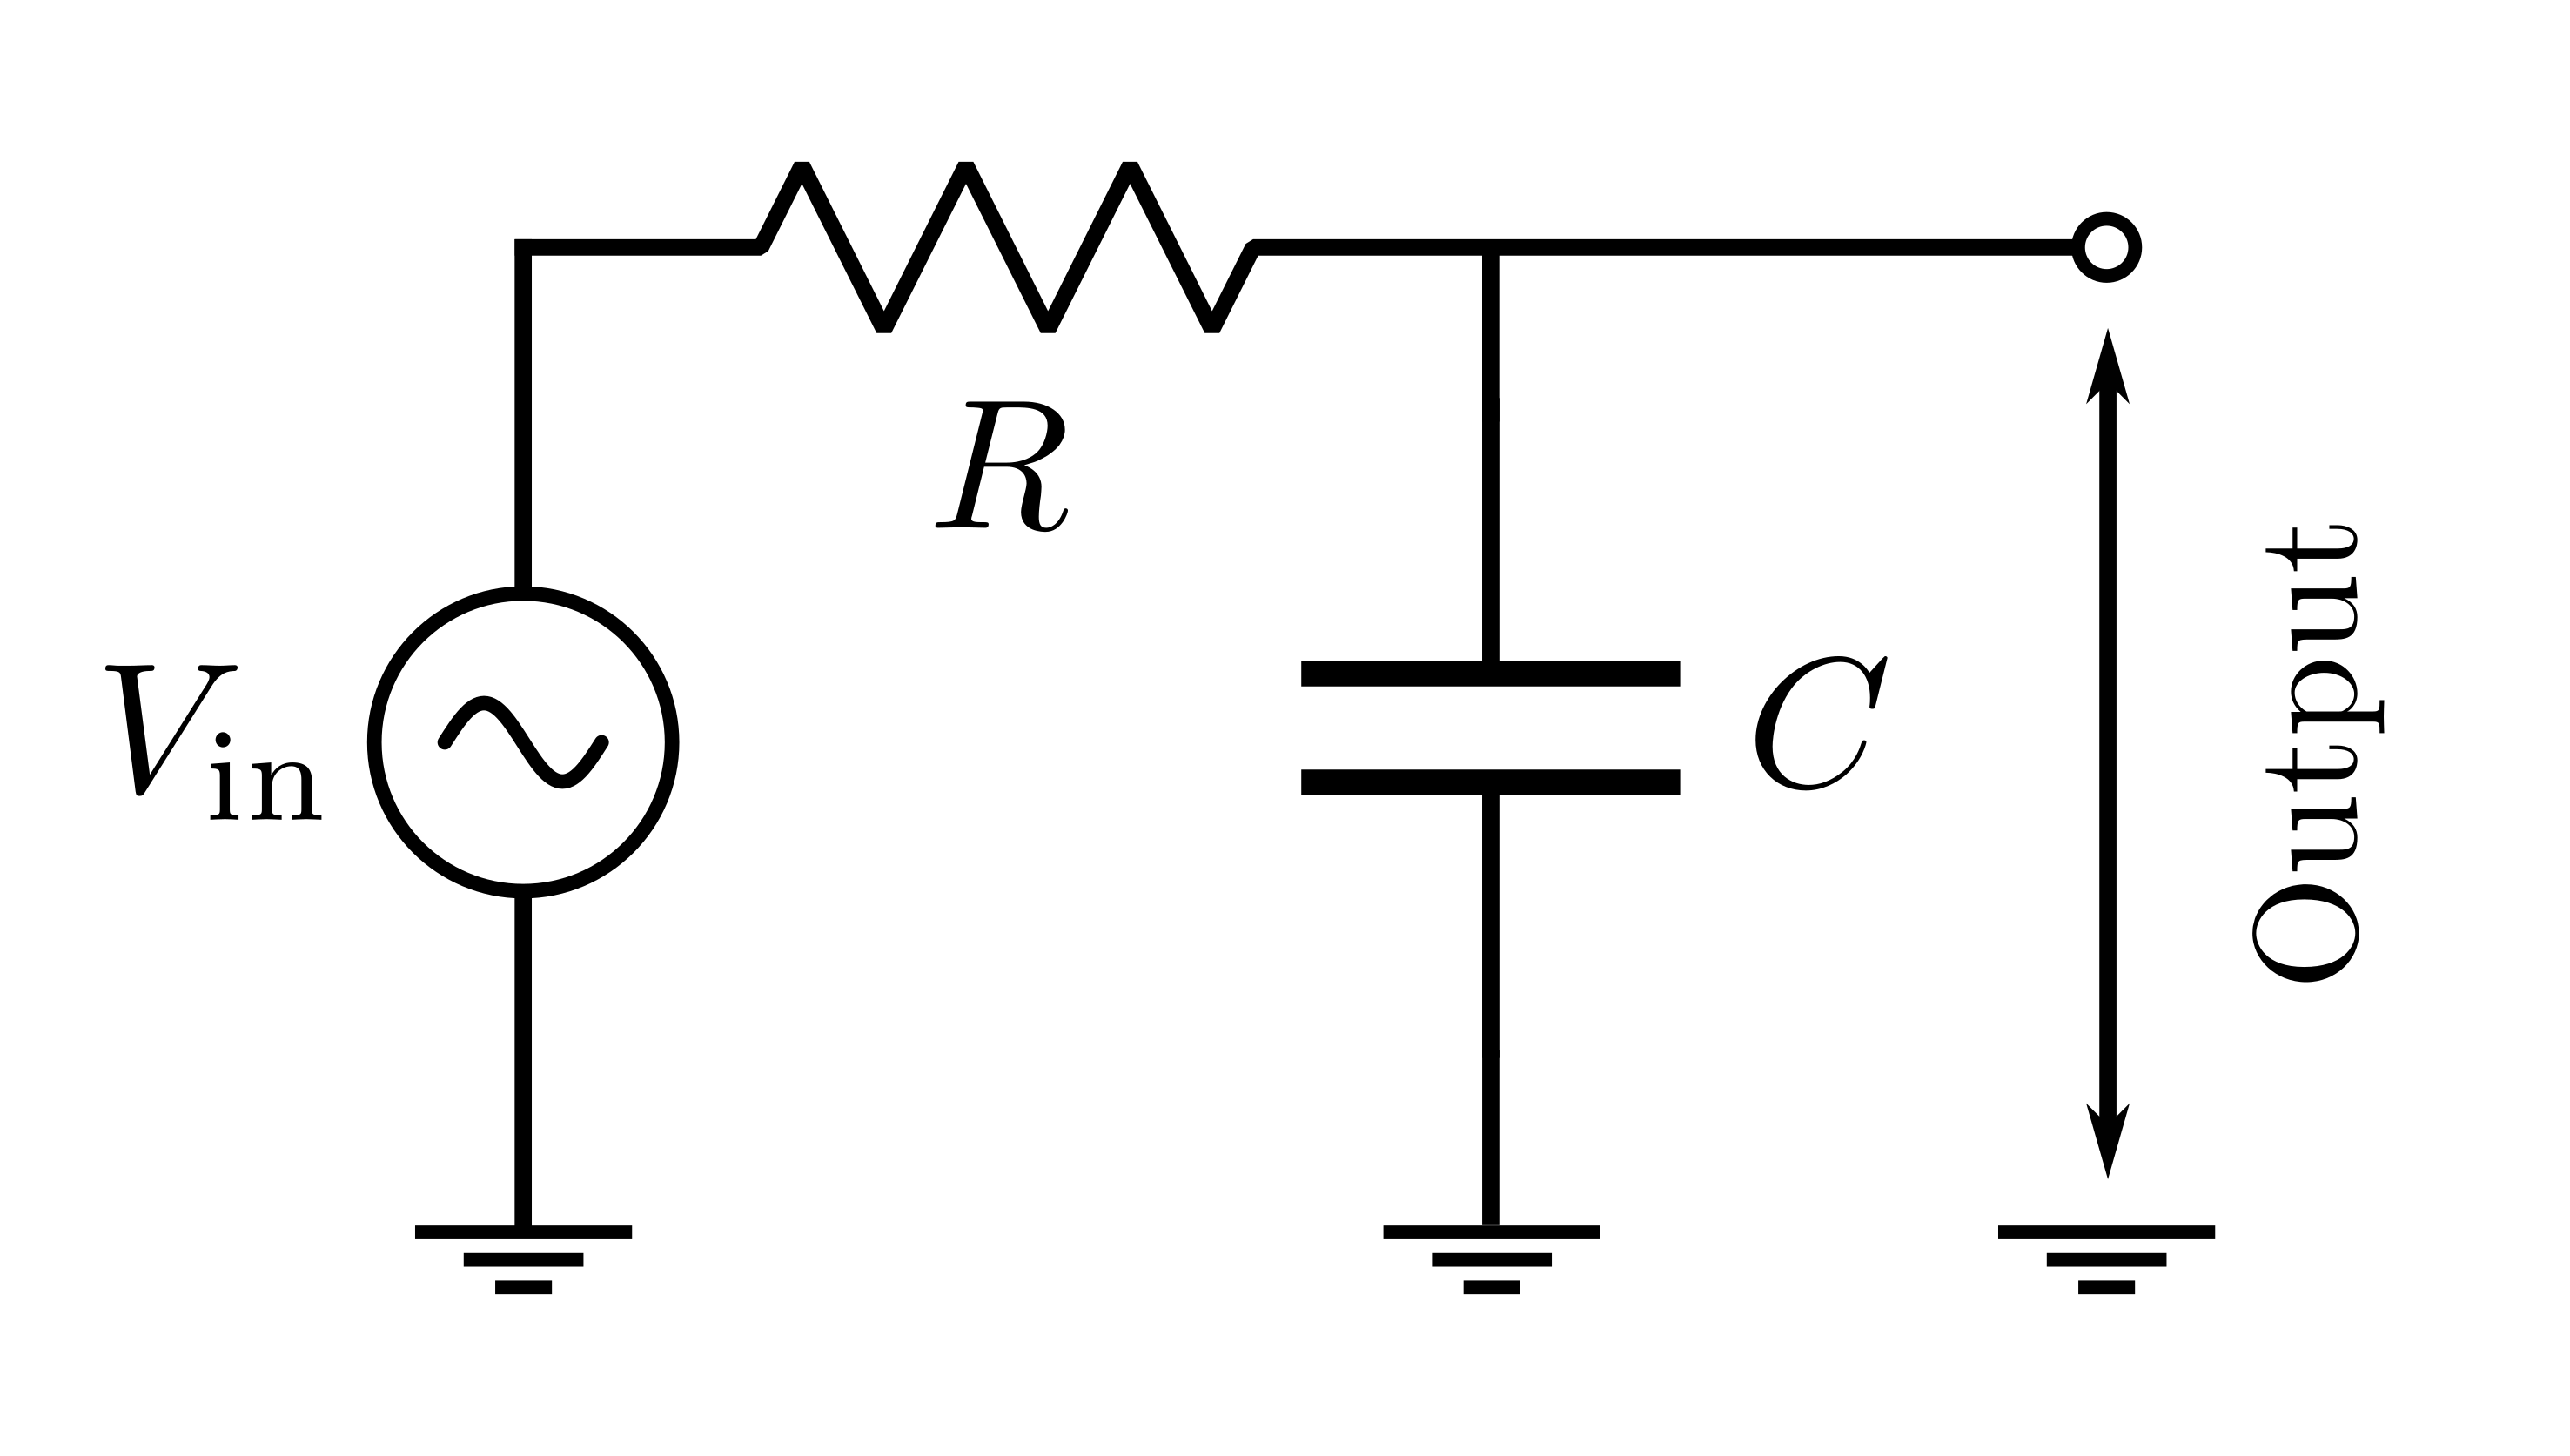
\includegraphics[width=\textwidth]{figs/electronics-circuits/RCLP.png}
        \caption{The RC integrator and low-pass filter}
        \label{fig:rc-lp}
    \end{subfigure}\hfill
    \begin{subfigure}[b]{0.45\textwidth}
        \centering
        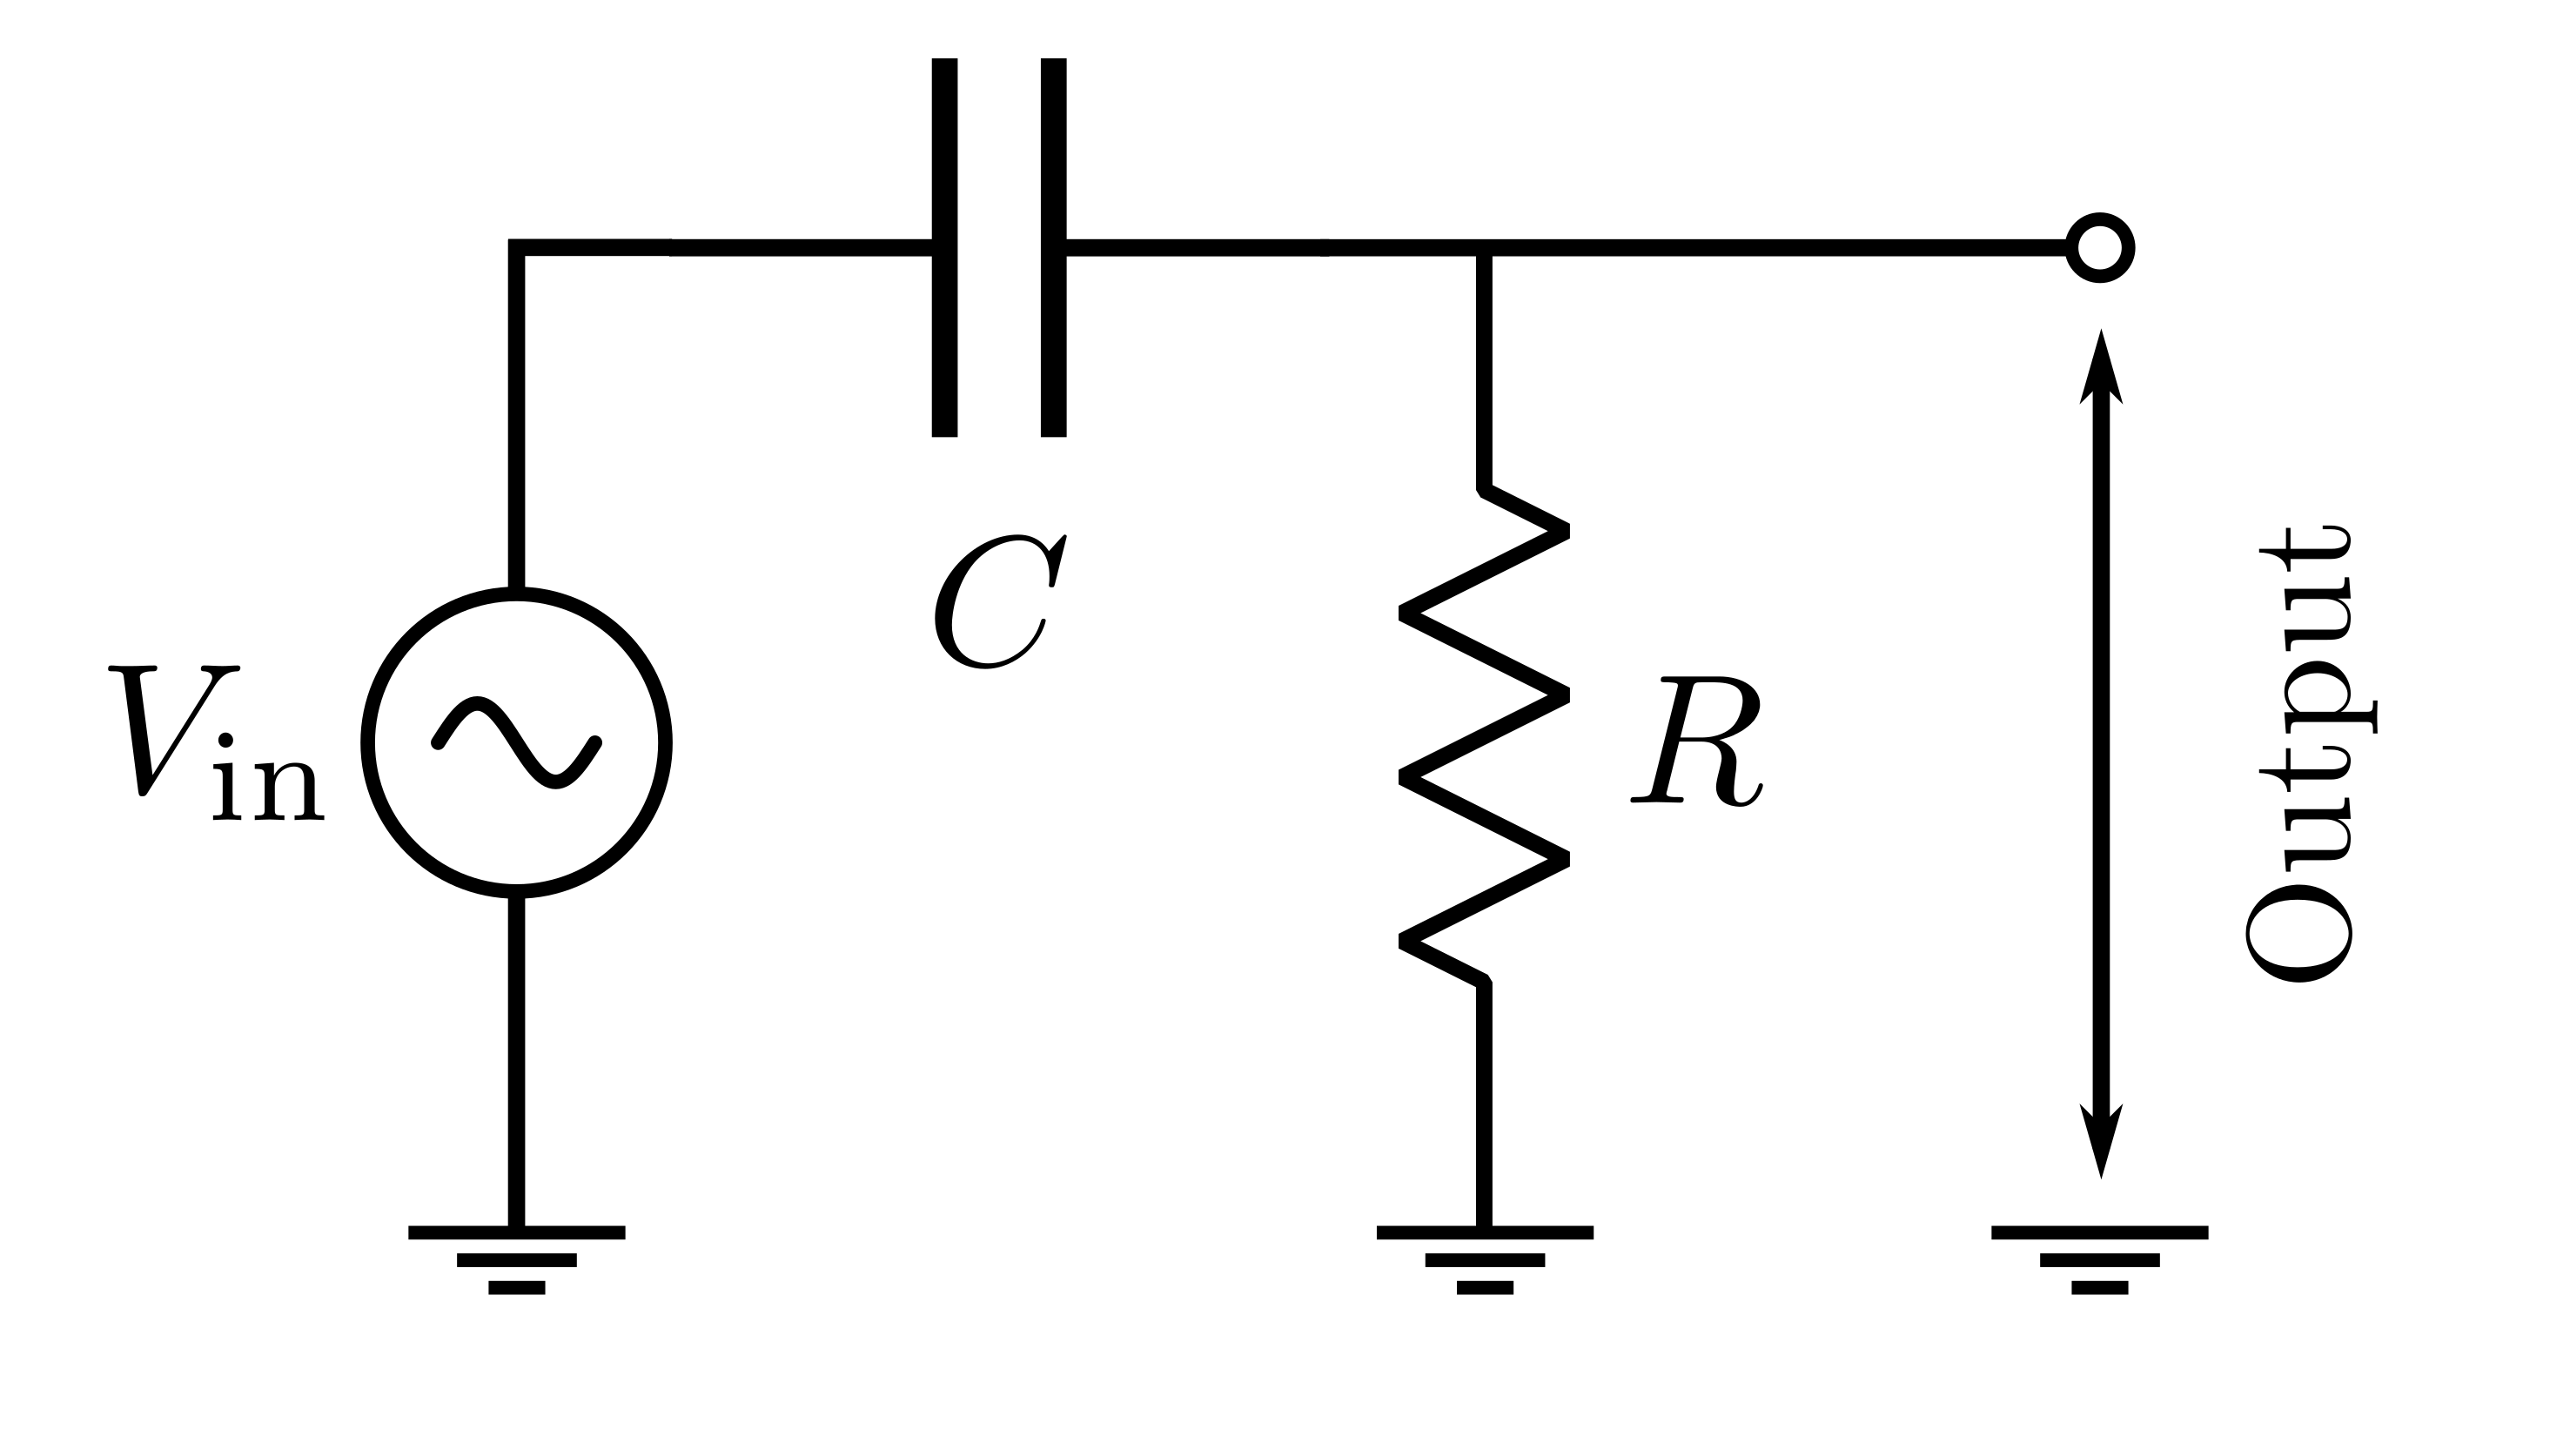
\includegraphics[width=\textwidth]{figs/electronics-circuits/RCHP.png}
        \caption{The RC differentiator and high-pass filter}
        \label{fig:rc-hp}
    \end{subfigure}
    \caption{Different possible configurations for an $RC$ circuit. In (a) we see the configuration that works both as a integrator and a low-pass filter, while in (b) we see the configuration that works both as a differentiator and a high-pass filter.}
    \label{fig:RC-configs}
\end{figure}

\subsection*{The RC circuit as a filter}

In our analysis so far, we have considered the time-series behaviour of our system: a time-varying signal can be either integrated or differentiated based on the $RC$ configuration. However, the above analysis has another interesting consequence. As we have seen above, in the case of the ``integrator'' configuration $V_R \approx V_\text{in}$. Thus the output voltage across the capacitor is essentially zero at high-frequencies. In other words, such a configuration \textsl{blocks} high frequencies when compared to low frequencies. When this occurs, we say that the $RC$ circuit is working as a \textsl{low-pass} filter, as it allows low frequencies to pass undisturbed, and attenuates high frequencies.

Similarly, in the ``differentiator'' configuration, we have seen that $V_C \approx V_\text{in}$, and therefore the output across the resistor is essentially zero at \textsl{low} frequencies. Therefore, in this particular configuration, high frequencies are allowed to pass essentially undisturbed, and low frequencies are attenuated.

Thus, given an $RC$ circuit we can construct a \textsl{cutoff} frequency $\omega_c = 1/RC$ such that for high-frequencies ($\omega \gg \omega_c$) one configuration -- Figure~(\ref{fig:rc-lp}) -- attenuates these frequencies, and the other -- Figure~(\ref{fig:rc-hp}) -- allows them to pass without modification.

\subsubsection*{Gain, decibels, and Bode plots}

In order to study the response of such filters, we define the concept of a ``gain'' of an electrical circuit. The gain of a circuit is just the ratio of the output to the input voltage. A gain of greater than one means the signal was amplified, while a gain of less than one means it was attenuated. It turns out that a log scale is much more convenient for talking about gains, and so by convention we define a unit called a ``bel'', which is an increase in power by 10 times,
\begin{equation}
    \text{gain in B} = \log_{10}\left( \frac{P_\text{out}}{P_\text{in}} \right).
\end{equation}
The bel is inconveniently large, and for historical reasons\footnote{The bel can be traced back to the old phone and telegraph system. Indeed, the unit was itself named after Alexander Graham Bell, the inventor of the telephone.} it was replaced by a smaller unit, the \textsl{deci}bel: one-tenth of a bel. The gain in units of decibel is 10 times the gain in units of bel,
\begin{equation}
    \text{gain in dB} = 10\,\, \text{ gain in B} = 10 \,\,\log_{10}\left( \frac{P_\text{out}}{P_\text{in}} \right).
\end{equation}
Now, as we have seen, we will be measuring voltages rather than power. For a resistive circuit, for example, we know that $P =V^2/R$, and so we can thus rewrite the earlier equation in terms of the ratio of voltages rather than the ratio of powers, since
\begin{equation}
    \text{gain in dB} = 10 \,\,\log_{10} \left( \frac{V^2_\text{out}}{V^2_\text{in}} \right) = 20 \,\log_{10} \left( \frac{V_\text{out}}{V_\text{in}} \right).
\end{equation}

Lastly, all the plots dealing with the gain are often ``Bode'' plots. In such plots, the $y-$axis is the gain, and the $x-$axis is the frequency in a log scale. This results in a log-log plot, since both the axes are logarithmic variables. We will not go into the reasons for using such plots here (although they are very interesting!) but will instead restrict ourselves to using them.


\subsubsection*{The low-pass and high-pass filters}

Let us now compute the ratio of the output voltage to the input voltage for a low-pass filter. In this configuration, the output voltage is the voltage across the capacitor, and so 
\begin{equation}
    \text{gain} = \frac{V_\text{out}}{V_\text{in}} = \frac{V_C}{V_\text{in}}.
\end{equation}

\begin{question}
    \textbf{Question:} Using the fact that $V_C = I z_C$, and the expression for the current in Equation~(\ref{eqn:RC-current}), show that 
    \begin{equation}
        \frac{V_C}{V_\text{in}} = \frac{1}{1 + i \omega R C}.
    \end{equation}

    \textbf{Question:} The actual gain is the real part of this. Using the fact that if $x$ is a real, then
    \begin{equation}
        \Re \left( \frac{1}{1 + i x }\right) = \frac{1}{\sqrt{1 + x^2}},
    \end{equation}
    % show that
    \begin{equation}
        \text{gain} = \dfrac{1}{\sqrt{1 + \omega^2 R^2 C^2}} = \frac{1}{\sqrt{1 + \left(\omega/\omega_c\right)^2}}.
    \end{equation}
    
\end{question}


Similarly, let us compute the same quantity for the high-pass filter. In this case, the output voltage is taken across the resistor, and therefore
\begin{equation}
    \text{gain} = \frac{V_\text{out}}{V_\text{in}} = \frac{V_R}{V_\text{in}}.
\end{equation}

\begin{question}
    \textbf{Question:} Using the same technique as in the previous question, show that 
    \begin{equation}
        \text{gain} = \dfrac{\omega R C}{\sqrt{1 + \omega^2 R^2 C^2}} = \frac{\left(\omega/\omega_c\right)}{\sqrt{1 + \left(\omega/\omega_c\right)^2}}.
    \end{equation}
\end{question}

The above equations for the gains of the low- and high-pass filters can be plotted. The results are shown in Figure~(\ref{fig:RC-bode}).

\begin{figure}[!htb]
    \centering
    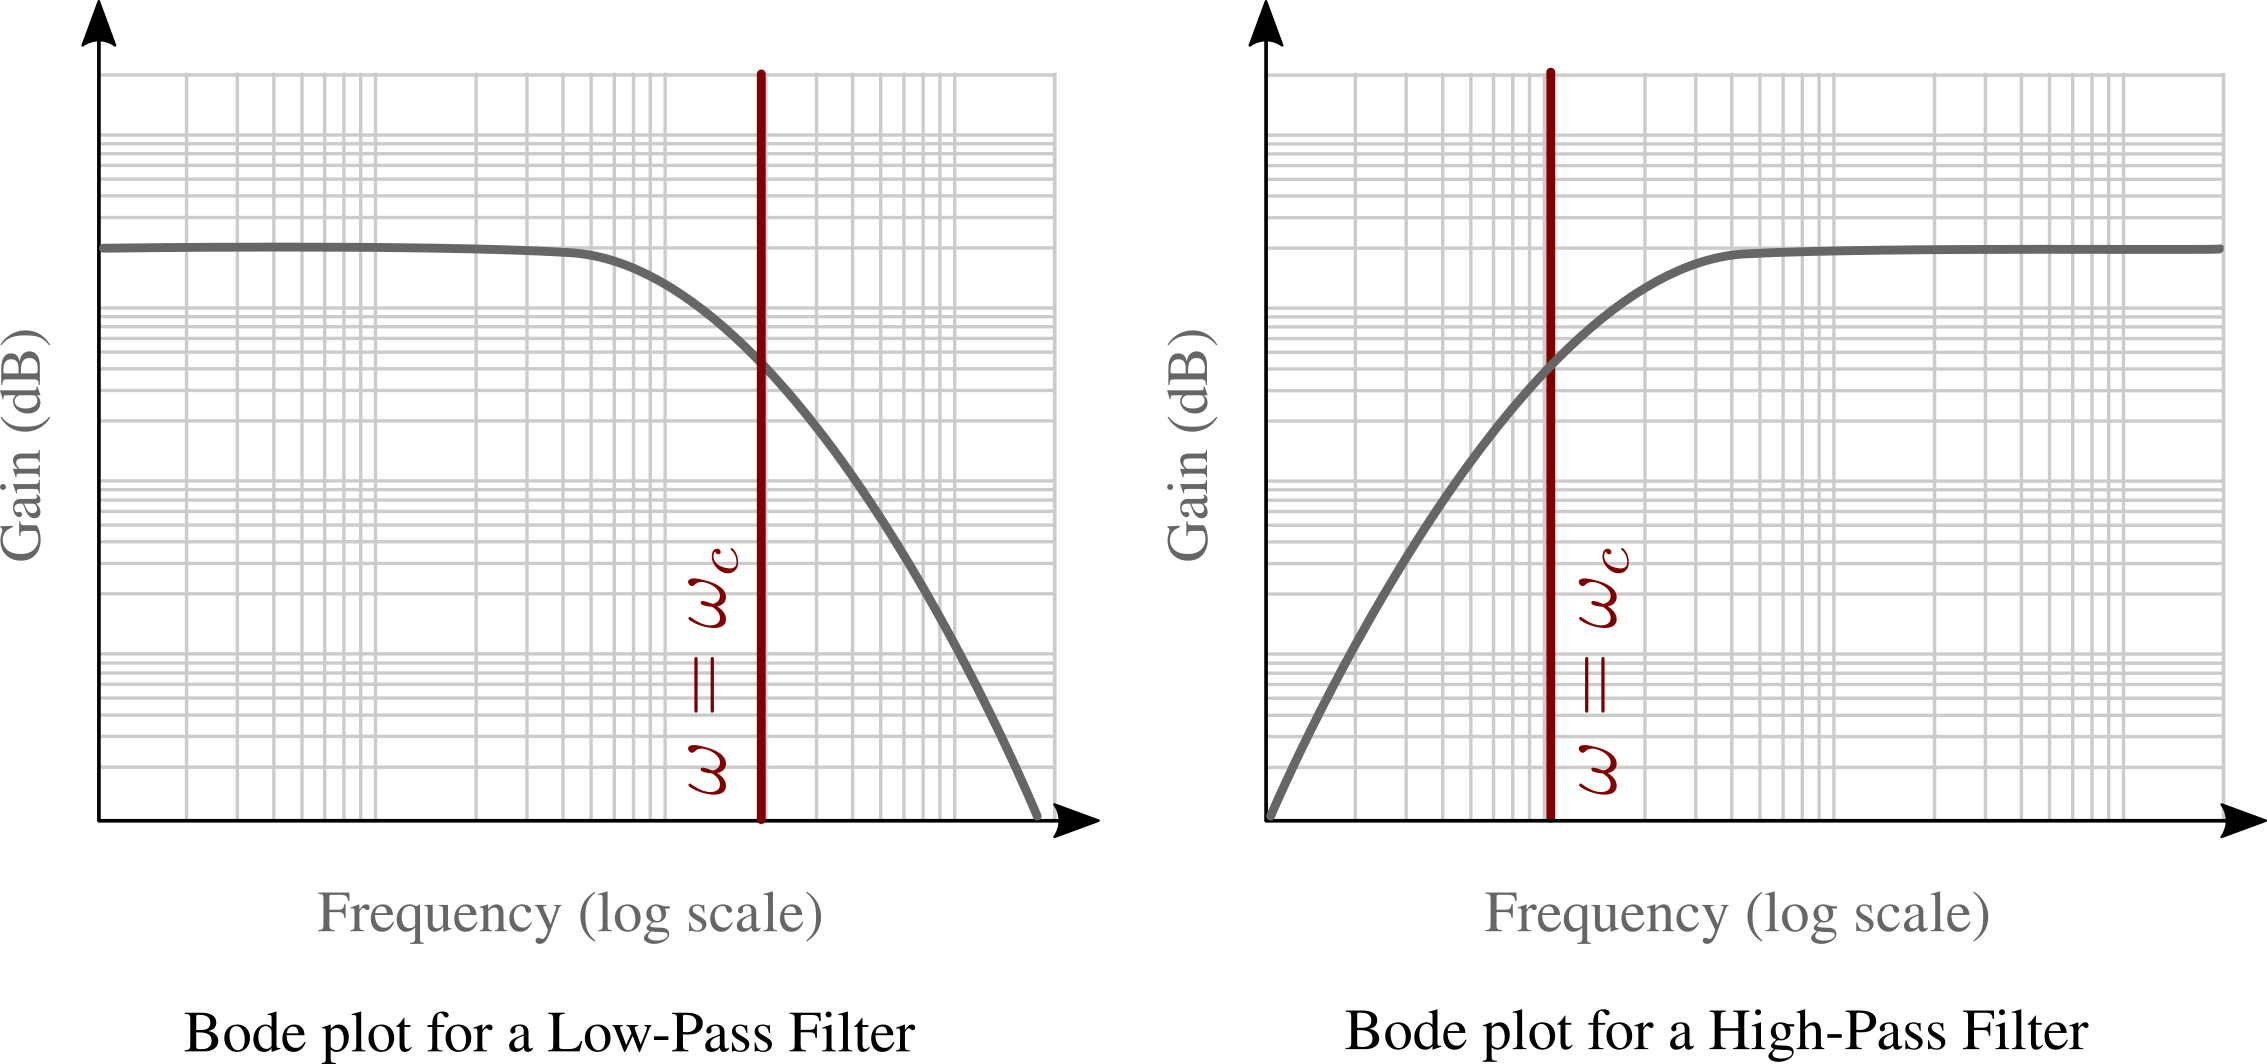
\includegraphics[width=0.9\textwidth]{figs/electronics-circuits/RC-gain.png}
    \caption{Bode plots for the low- and high-pass filters. In both cases, $\omega = \omega_c$ marks a ``knee'' in the graph. In the case of the low-pass filter, the gain (in dB) is initially constant and starts to decrease sharply as $\omega$ becomes greater than $\omega_c$. The converse is true for the high-pass filter: the gain increases sharply reaches a plateau when $\omega$ is greater than $\omega_c$.}
    \label{fig:RC-bode}
\end{figure}

\begin{imp}
    We have discussed different applications of the two circuits shown in Figure~(\ref{fig:RC-configs}), and it is easy to get confused about which configuration can be used for which. A summary at this point would be useful:

    \centering

    \begin{tabular}{@{}cccc@{}}
    \toprule
    \textbf{}                                                            \textbf{Circuit} & \textbf{Output}   & \textbf{Time-domain}  & \textbf{Frequency-domain} \\ \midrule
    \begin{tabular}[c]{@{}c@{}}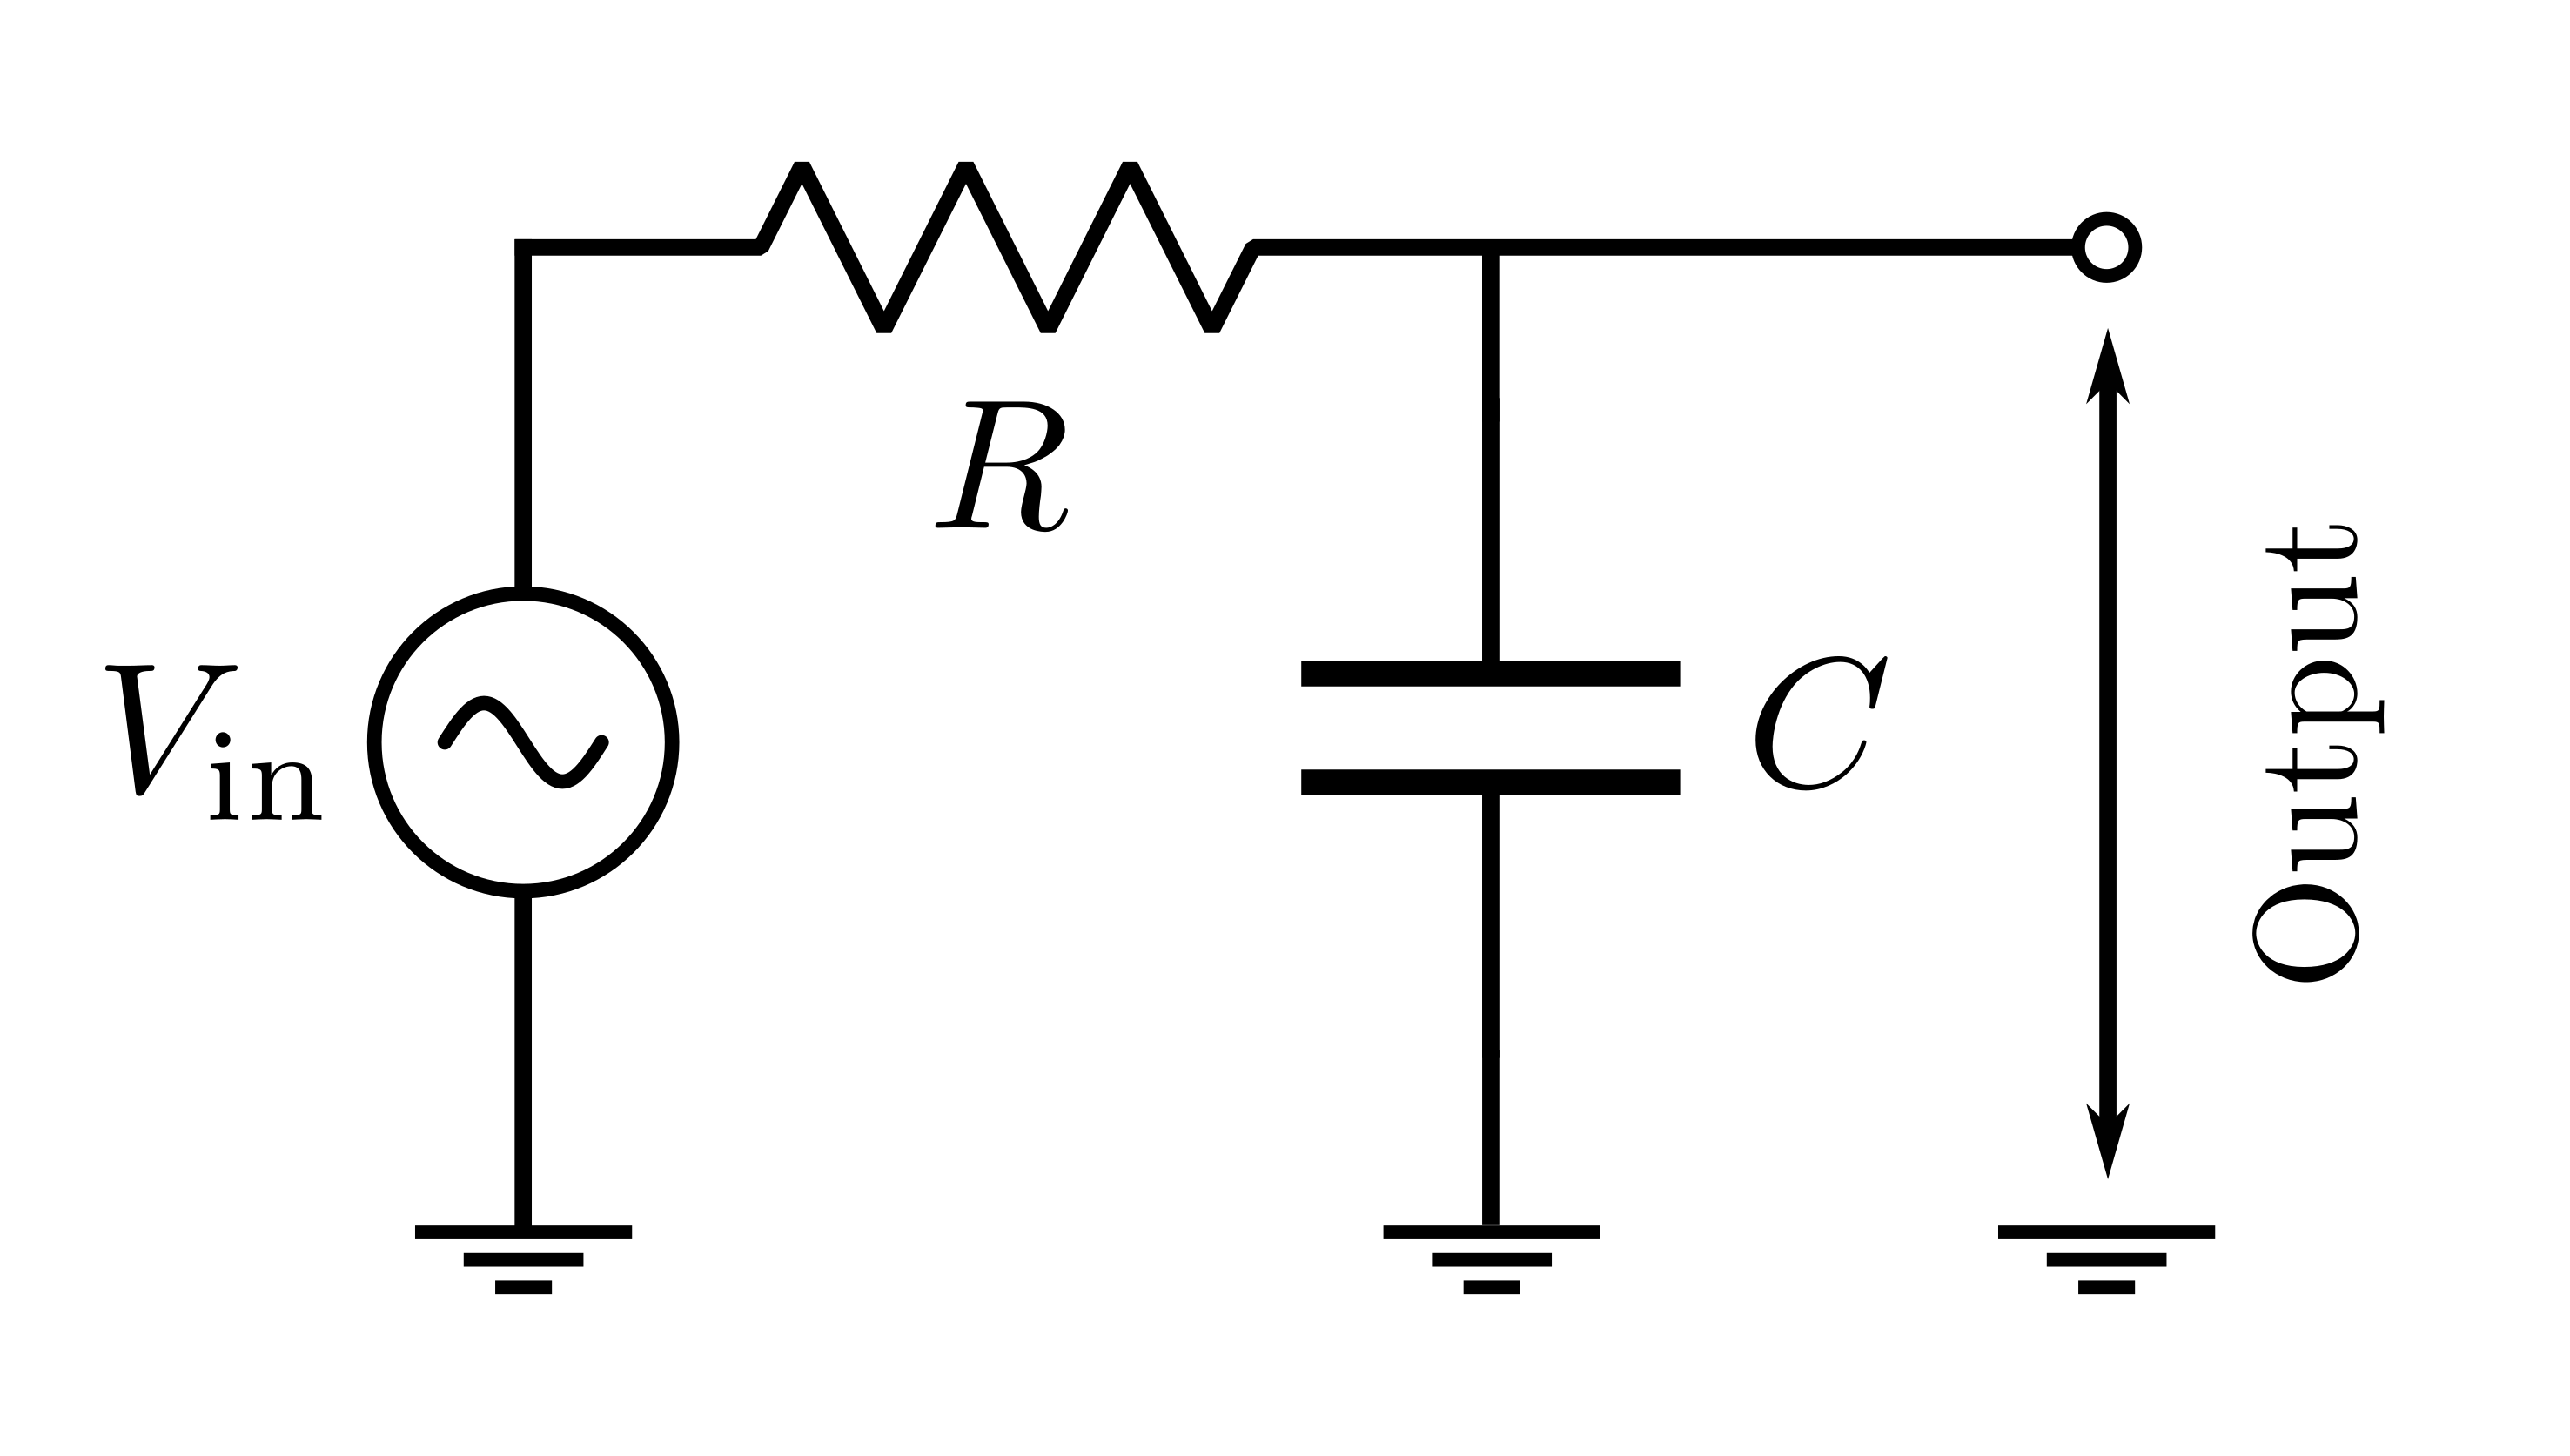
\includegraphics[width=0.23\textwidth]{figs/electronics-circuits/RCLP.png}\end{tabular} &
    \begin{tabular}[c]{@{}c@{}} Across capacitor\\ (see Figure~(\ref{fig:rc-lp}))\end{tabular} & \begin{tabular}[c]{@{}c@{}}Integrator\\ when $\omega \ll \omega_c$\end{tabular}     & Low-pass filter           \\
    \begin{tabular}[c]{@{}c@{}}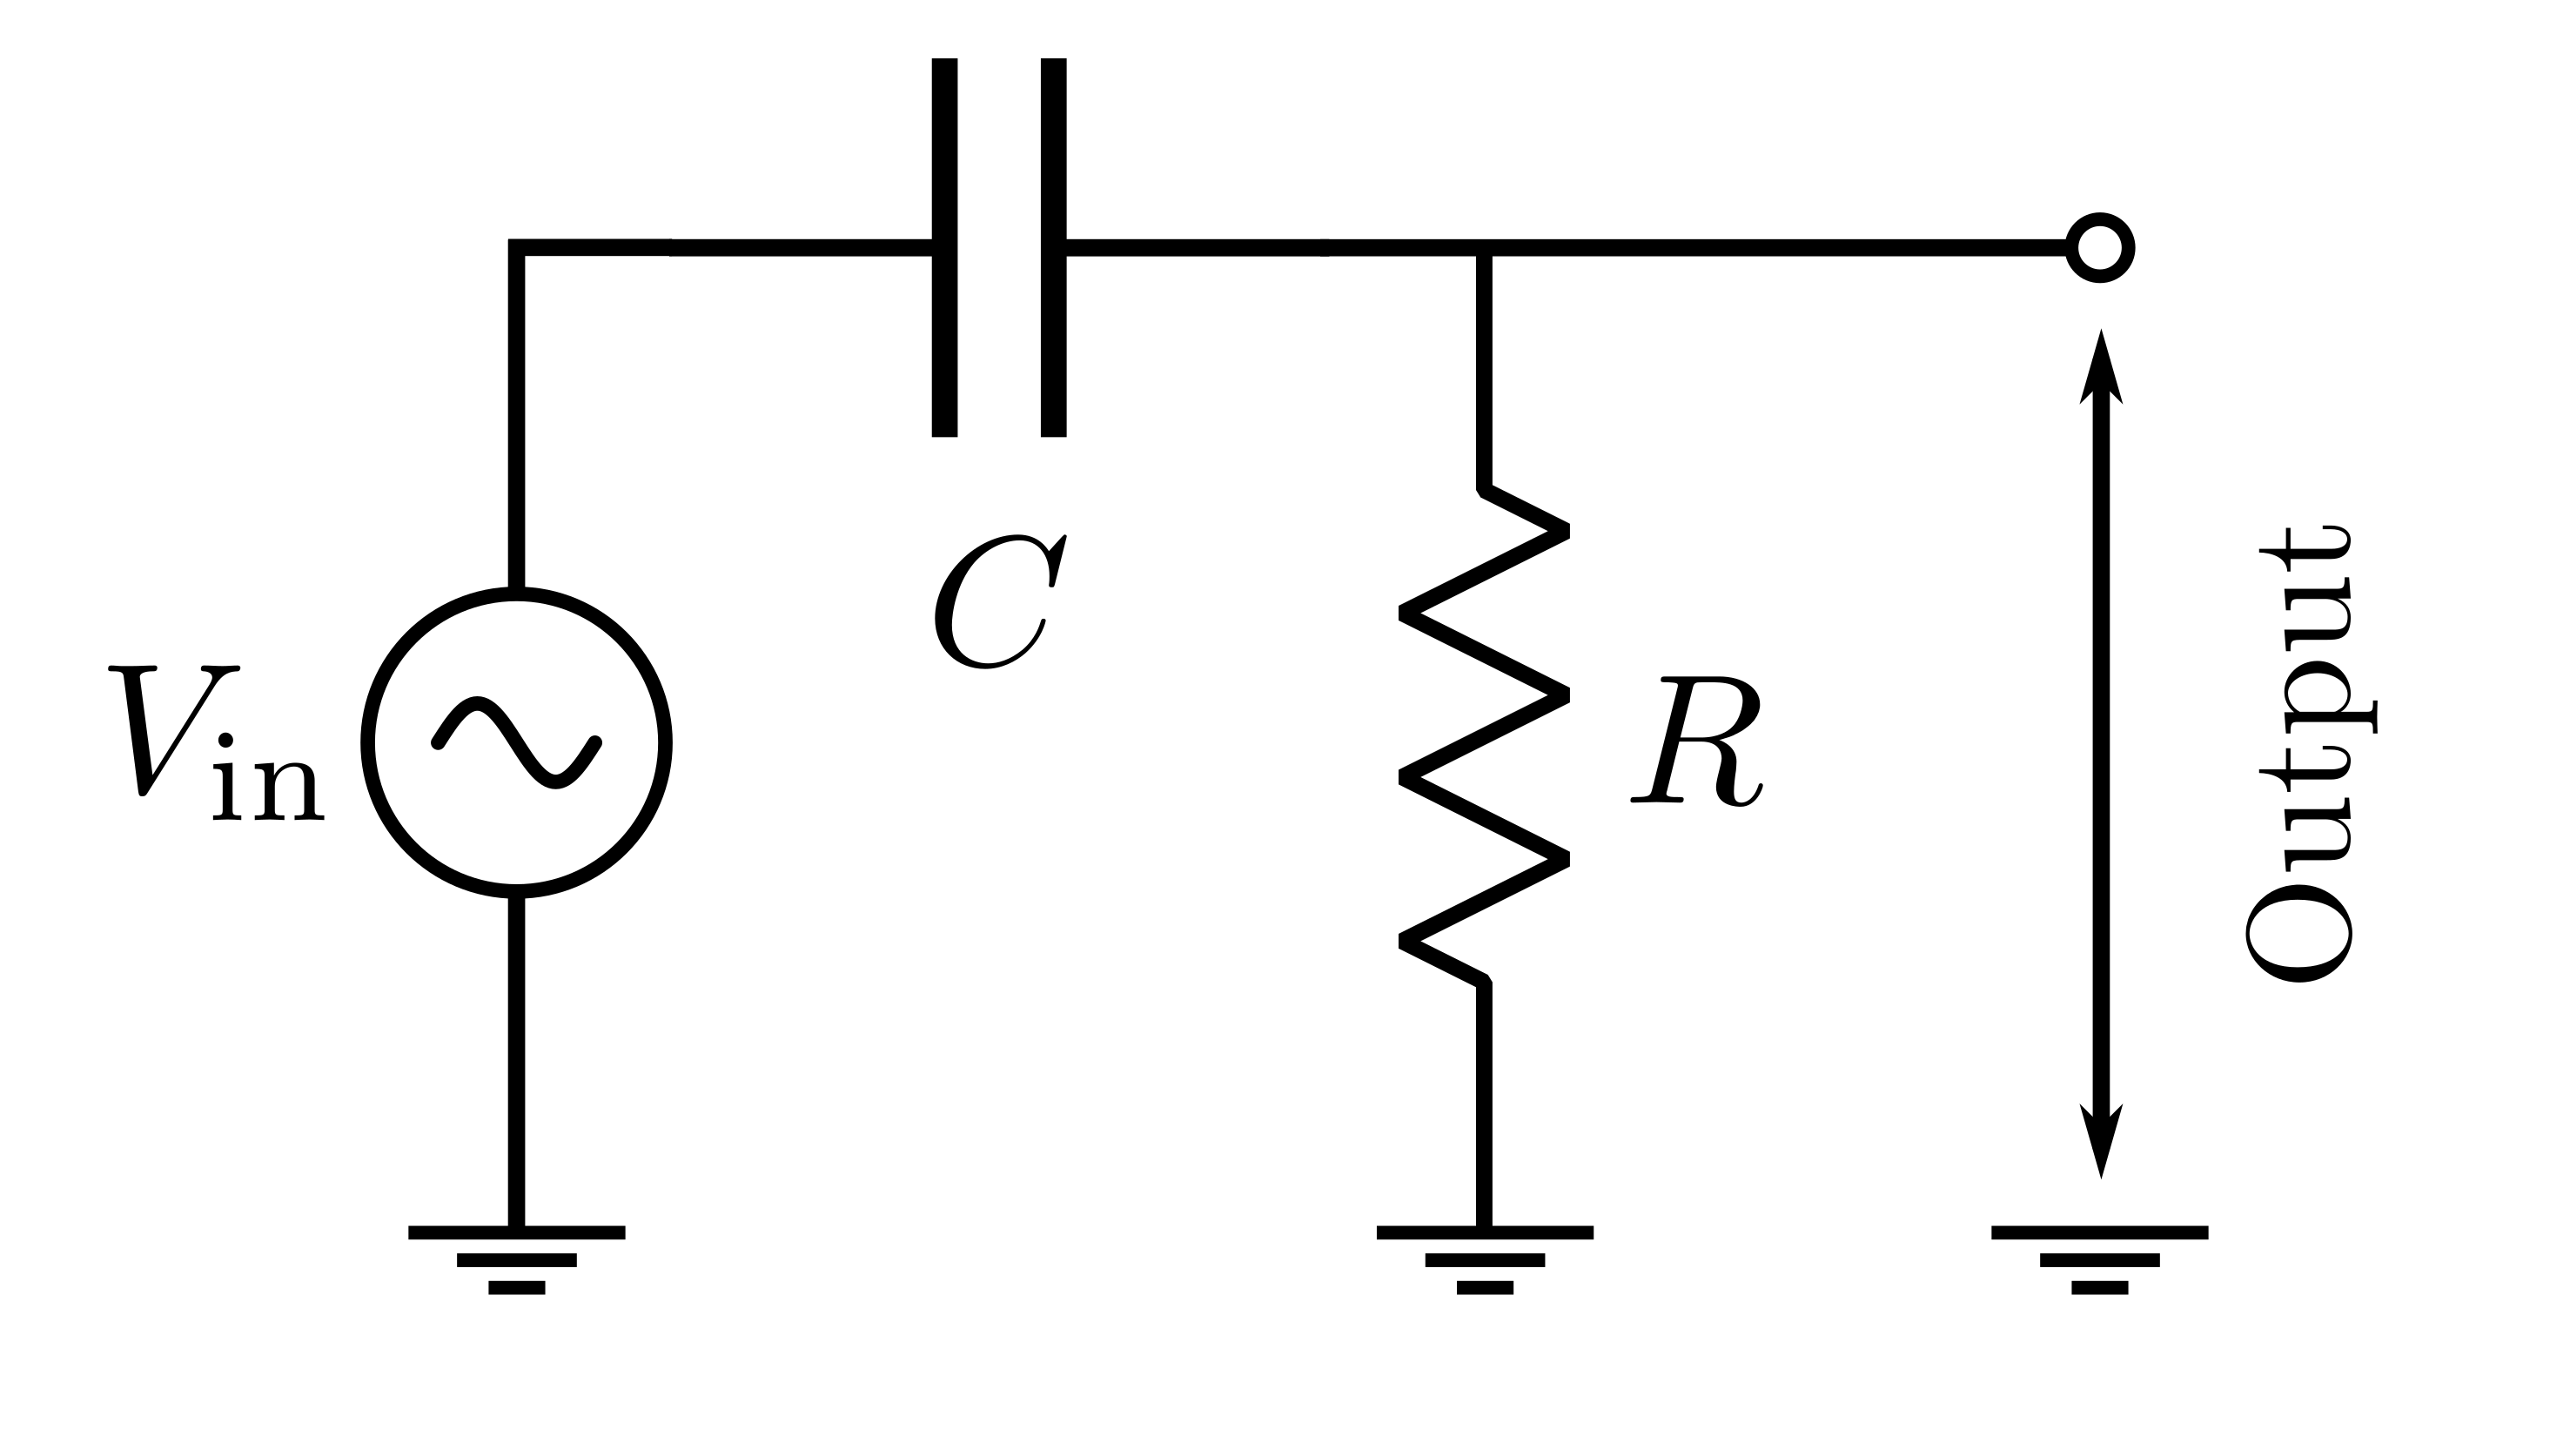
\includegraphics[width=0.23\textwidth]{figs/electronics-circuits/RCHP.png}\end{tabular} & \begin{tabular}[c]{@{}c@{}} Across resistor\\ (see Figure~(\ref{fig:rc-hp})\end{tabular}  & \begin{tabular}[c]{@{}c@{}}Differentiator\\ when $\omega \gg \omega_c$\end{tabular} & High-pass filter          \\ \bottomrule
    \end{tabular}
    
    
\end{imp}


\subsection*{The LCR circuit}

\begin{figure}[!htb]
    \centering
    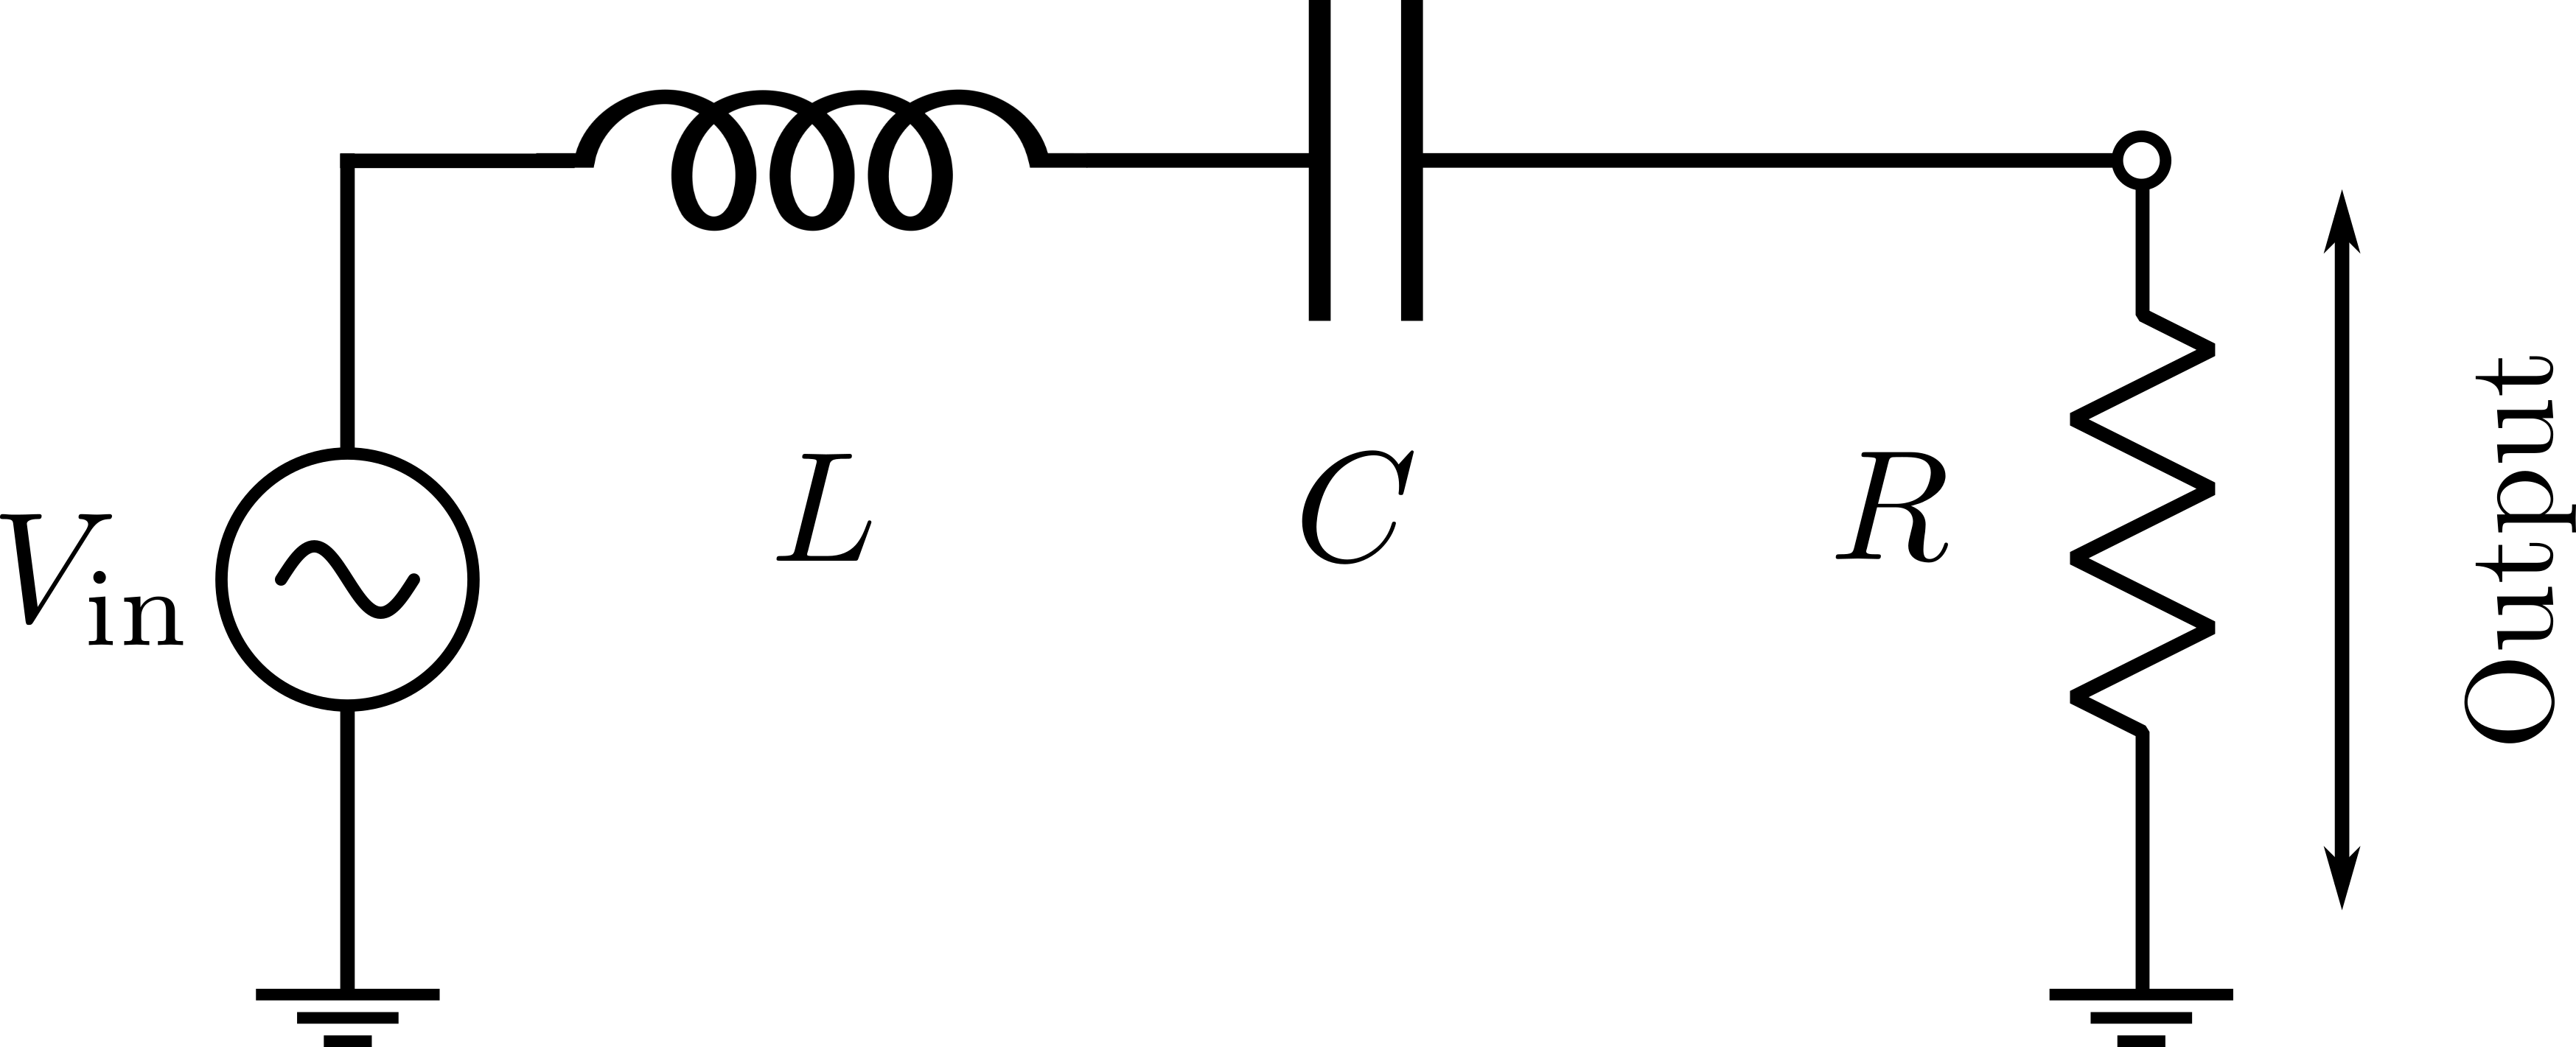
\includegraphics[width=0.65\textwidth]{figs/electronics-circuits/LCRSeries.png}
    \caption{A series $LCR$ circuit. The inductor, capacitor, and resistor are attached to an AC power supply, and the output voltage is taken across the resistor. }
    \label{fig:lcr-series}
\end{figure}

We are now ready to study a more complicated circuit: consider a series combination of an inductor, capacitor, and resistor, as shown in Figure~(\ref{fig:lcr-series}). As with the $RC$ circuit, we first study the natural response of this system: how does it behave in the absence of any external driving force. Using Kirchoff's law, you should be able to show that since the potential drop across the various components in the closed circuit loop is zero, we have
\begin{equation}
    L \dv{I}{t} + R I + \frac{Q}{C} = 0.
\end{equation}

In itself, this equation may not look too familiar to you, but if you divide it by $L$ and take a derivative of the left-hand side with respect to time, you should be able to see that the equation becomes very familiar:
\begin{equation}
    \dv[2]{I}{t} + \gamma \dv{I}{t} + \omega_0^2 I = 0.
\end{equation}

This is just the differential equation for a damped harmonic oscillator with natural frequency $\omega_0$ and a damping coefficient of $\gamma$.

\begin{question}
    \textbf{Question:} Show that 
    \begin{equation}
        \omega_0 = \frac{1}{\sqrt{LC}}, \quad \quad \text{and} \quad \quad \gamma = \frac{R}{L}.
    \end{equation}
\end{question}

The analogy with the damped harmonic oscillator means that the form of this differential equation already allows us to draw some important conclusions:
\begin{itemize}
    \item If the resistance is not too high (i.e. if $\gamma < 2 \omega_0$ or $R < 2 \sqrt{L/C}$) the current in the circuit executes damped harmonic oscillations of the form
    \begin{equation}
        I(t) = I_0 e^{-\gamma t/2} \cos(\omega_1 t - \varphi),
    \end{equation}

    where $I_0$ and $\varphi$ are constants set by the initial conditions, and $\omega_1 = \sqrt{\omega_0^2 - \gamma^2/4}$.

    \item For values of resistance greater than $2 \sqrt{L/C}$, the system does not naturally exhibit oscillations, as is considered to be \textsl{overdamped}.

    \item The resistance plays the role of the dissipative term, allowing the system to lose energy. The inductance plays the role of the mass, and the capacitance the role of the spring-constant.
\end{itemize}

Introducing an AC signal to such a system is equivalent to driving a damped harmonic oscillator. Therefore, we should expect to see phenomena like resonance that you should already be familiar with from your study of mechanical systems.

\subsection*{Resonance in an $LCR$ oscillator}
Consider an $LCR$ circuit of some natural frequency $\omega_0$ being driven by an external AC frequency of $\omega$. As before, we consider that the voltage and current are both oscillating at the same frequency $\omega$. We can easily compute the net impedance of our series $LCR$ circuit as
\begin{equation}
    \begin{aligned}
        z &= z_L + z_C + z_R,\\
          &= i\omega L + \frac{1}{i\omega C} + R,\\ 
          &= R + i \left( \omega L - \frac{1}{\omega C} \right).
    \end{aligned}
\end{equation}

The current in this circuit is thus simply given by 
\begin{equation}
    I = \frac{V_\text{in}}{z} = \frac{V_\text{in}}{R + i  \left( \omega L - \dfrac{1}{\omega C} \right) }.
\end{equation}

\begin{question}
    \textbf{Question:} Show that the oscillator will draw the highest current from the power supply when 
    \begin{equation}
        \omega L = \frac{1}{\omega C}, \quad \iff \quad \omega = \frac{1}{\sqrt{LC}} = \omega_0. 
    \end{equation}

    This is called \textsl{resonance}.

    \textbf{Question:} Show that for such a ``series'' $LCR$ circuit (i) the net impedance is $0$ at both $\omega \to 0$ and $\omega\to\infty$, and (ii) at resonance, the net impedance is $z=R$.
\end{question}

Thus, when $\omega = \omega_0$, the impedance of the system is minimum and consequently, the system draws the greatest power from the power supply. As one moves away from $\omega=\omega_0$ on either side, the current drawn by the system reduces. We thus get a ``band'' over which the current is large, and beyond which the current falls rapidly. 

% The way that this happens depends on the \textsl{quality factor} of our oscillator, defined by
% \begin{equation}
%     \mathcal{Q} = \frac{\omega_0}{\gamma} = \frac{1}{R}\sqrt{\frac{L}{C}}.
% \end{equation}

% Clearly, when $R\to0$, the quality factor of 

The configuration shown in Figure~(\ref{fig:lcr-series}) is of course only one of many possible ways in which inductors, capacitors, and resistors can be combined. Another possible combination is to keep the components in \textsl{parallel}. One such configuration, known as a \textsl{tank} circuit, is shown in Figure~(\ref{fig:lcr-parallel}). 

\begin{figure}[!htb]
    \centering
    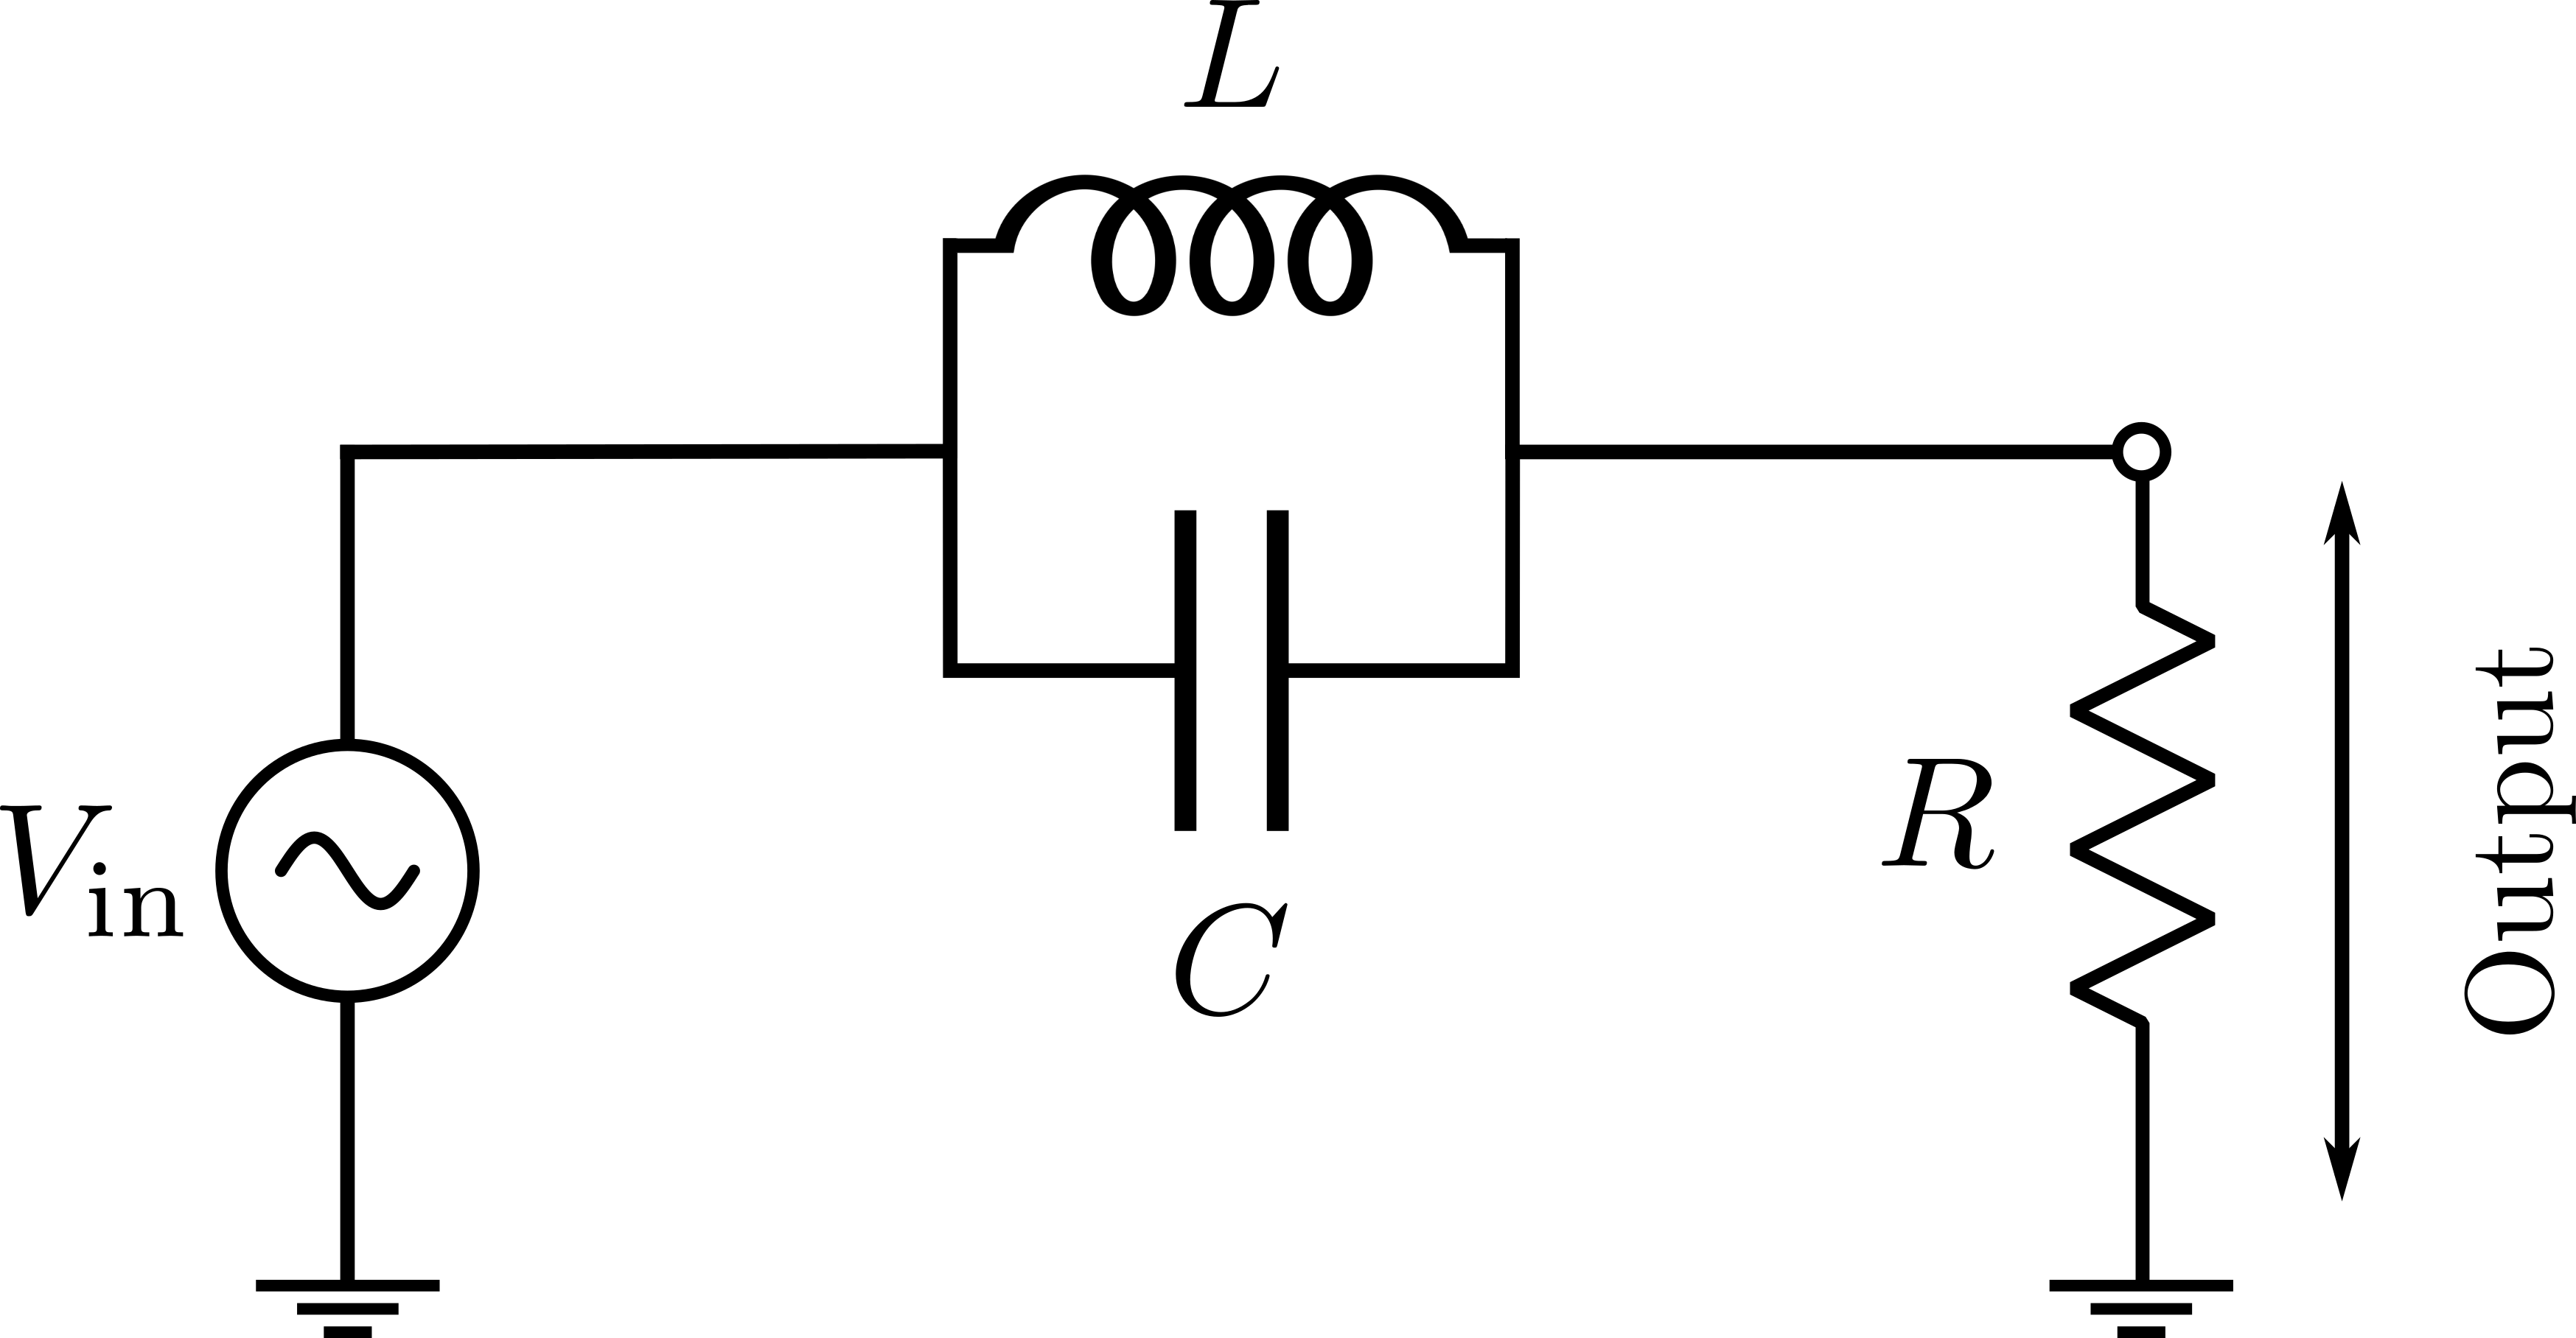
\includegraphics[width=0.65\textwidth]{figs/electronics-circuits/LCRParallel.png}
    \caption{One possible parallel configuration, known as a \textsl{tank} circuit. The inductor and the capacitor are connected in parallel, and the resistor is attached in series. An AC power supply is connected across the circuit, and the output voltage is taken across the resistor. }
    \label{fig:lcr-parallel}
\end{figure}

\begin{question}
    \textbf{Question:} As before, show that resonance occurs when $\omega = \omega_0$, just as in the series $LCR$ circuit.
    
    \textbf{Question:} Show that in the tank circuit (i) the net impedance is $0$ at both $\omega \to 0$ and $\omega\to\infty$, and (ii) at resonance, the net impedance is infinite. What does this mean for the current at resonance?
\end{question}


\subsubsection*{Phase shift around resonance}

Let us now understand exactly what happens around resonance. Consider the series $LCR$ circuit. As can be seen, resonance occurs when the complex part of the impedance goes to zero. In this case, the impedance is purely real -- the circuit is a pure resistor. Thus, when resonance occurs in such a circuit, the effect of the capacitor is exactly cancelled out by the effect of the inductor. However, as we have seen earlier, the inductor causes the current to lag behind the input voltage by a phase of $\pi/2$, while the capacitor causes the current to \textsl{lead} the voltage by the same phase of $\pi/2$. Therefore, at resonance, we would expect the current to be exactly in phase with the input voltage!

This can be detected by plotting a graph of the voltage against the current. Since for a sinusoidal signal these functions are in general out of phase at some arbitrary frequency $\omega \neq \omega_0$, we get what is known as a ``Lissajous'' figure: a superposition of two perpendicular out-of-phase sinusoidally varying functions, as shown in Figure~(\ref{fig:lissajous}). Since our frequencies are all the same, our Lissajous figures are all ellipses. The Lissajous figure can be used to determine the \textsl{phase} difference between the two signals by measuring the quantities $a$ and $b$ shown in Figure~(\ref{fig:lissajous}), where $a$ is the (positive) value of $x$ when $y=0$, and $b$ is the maximum value of $x$. 

The Lissajous figure can also be used to detect resonance, since at resonance the phase-difference is zero, meaning that the ellipse simply becomes a straight line. In other words, at resonance $a\to 0$.

\begin{figure}[!htb]
    \centering
    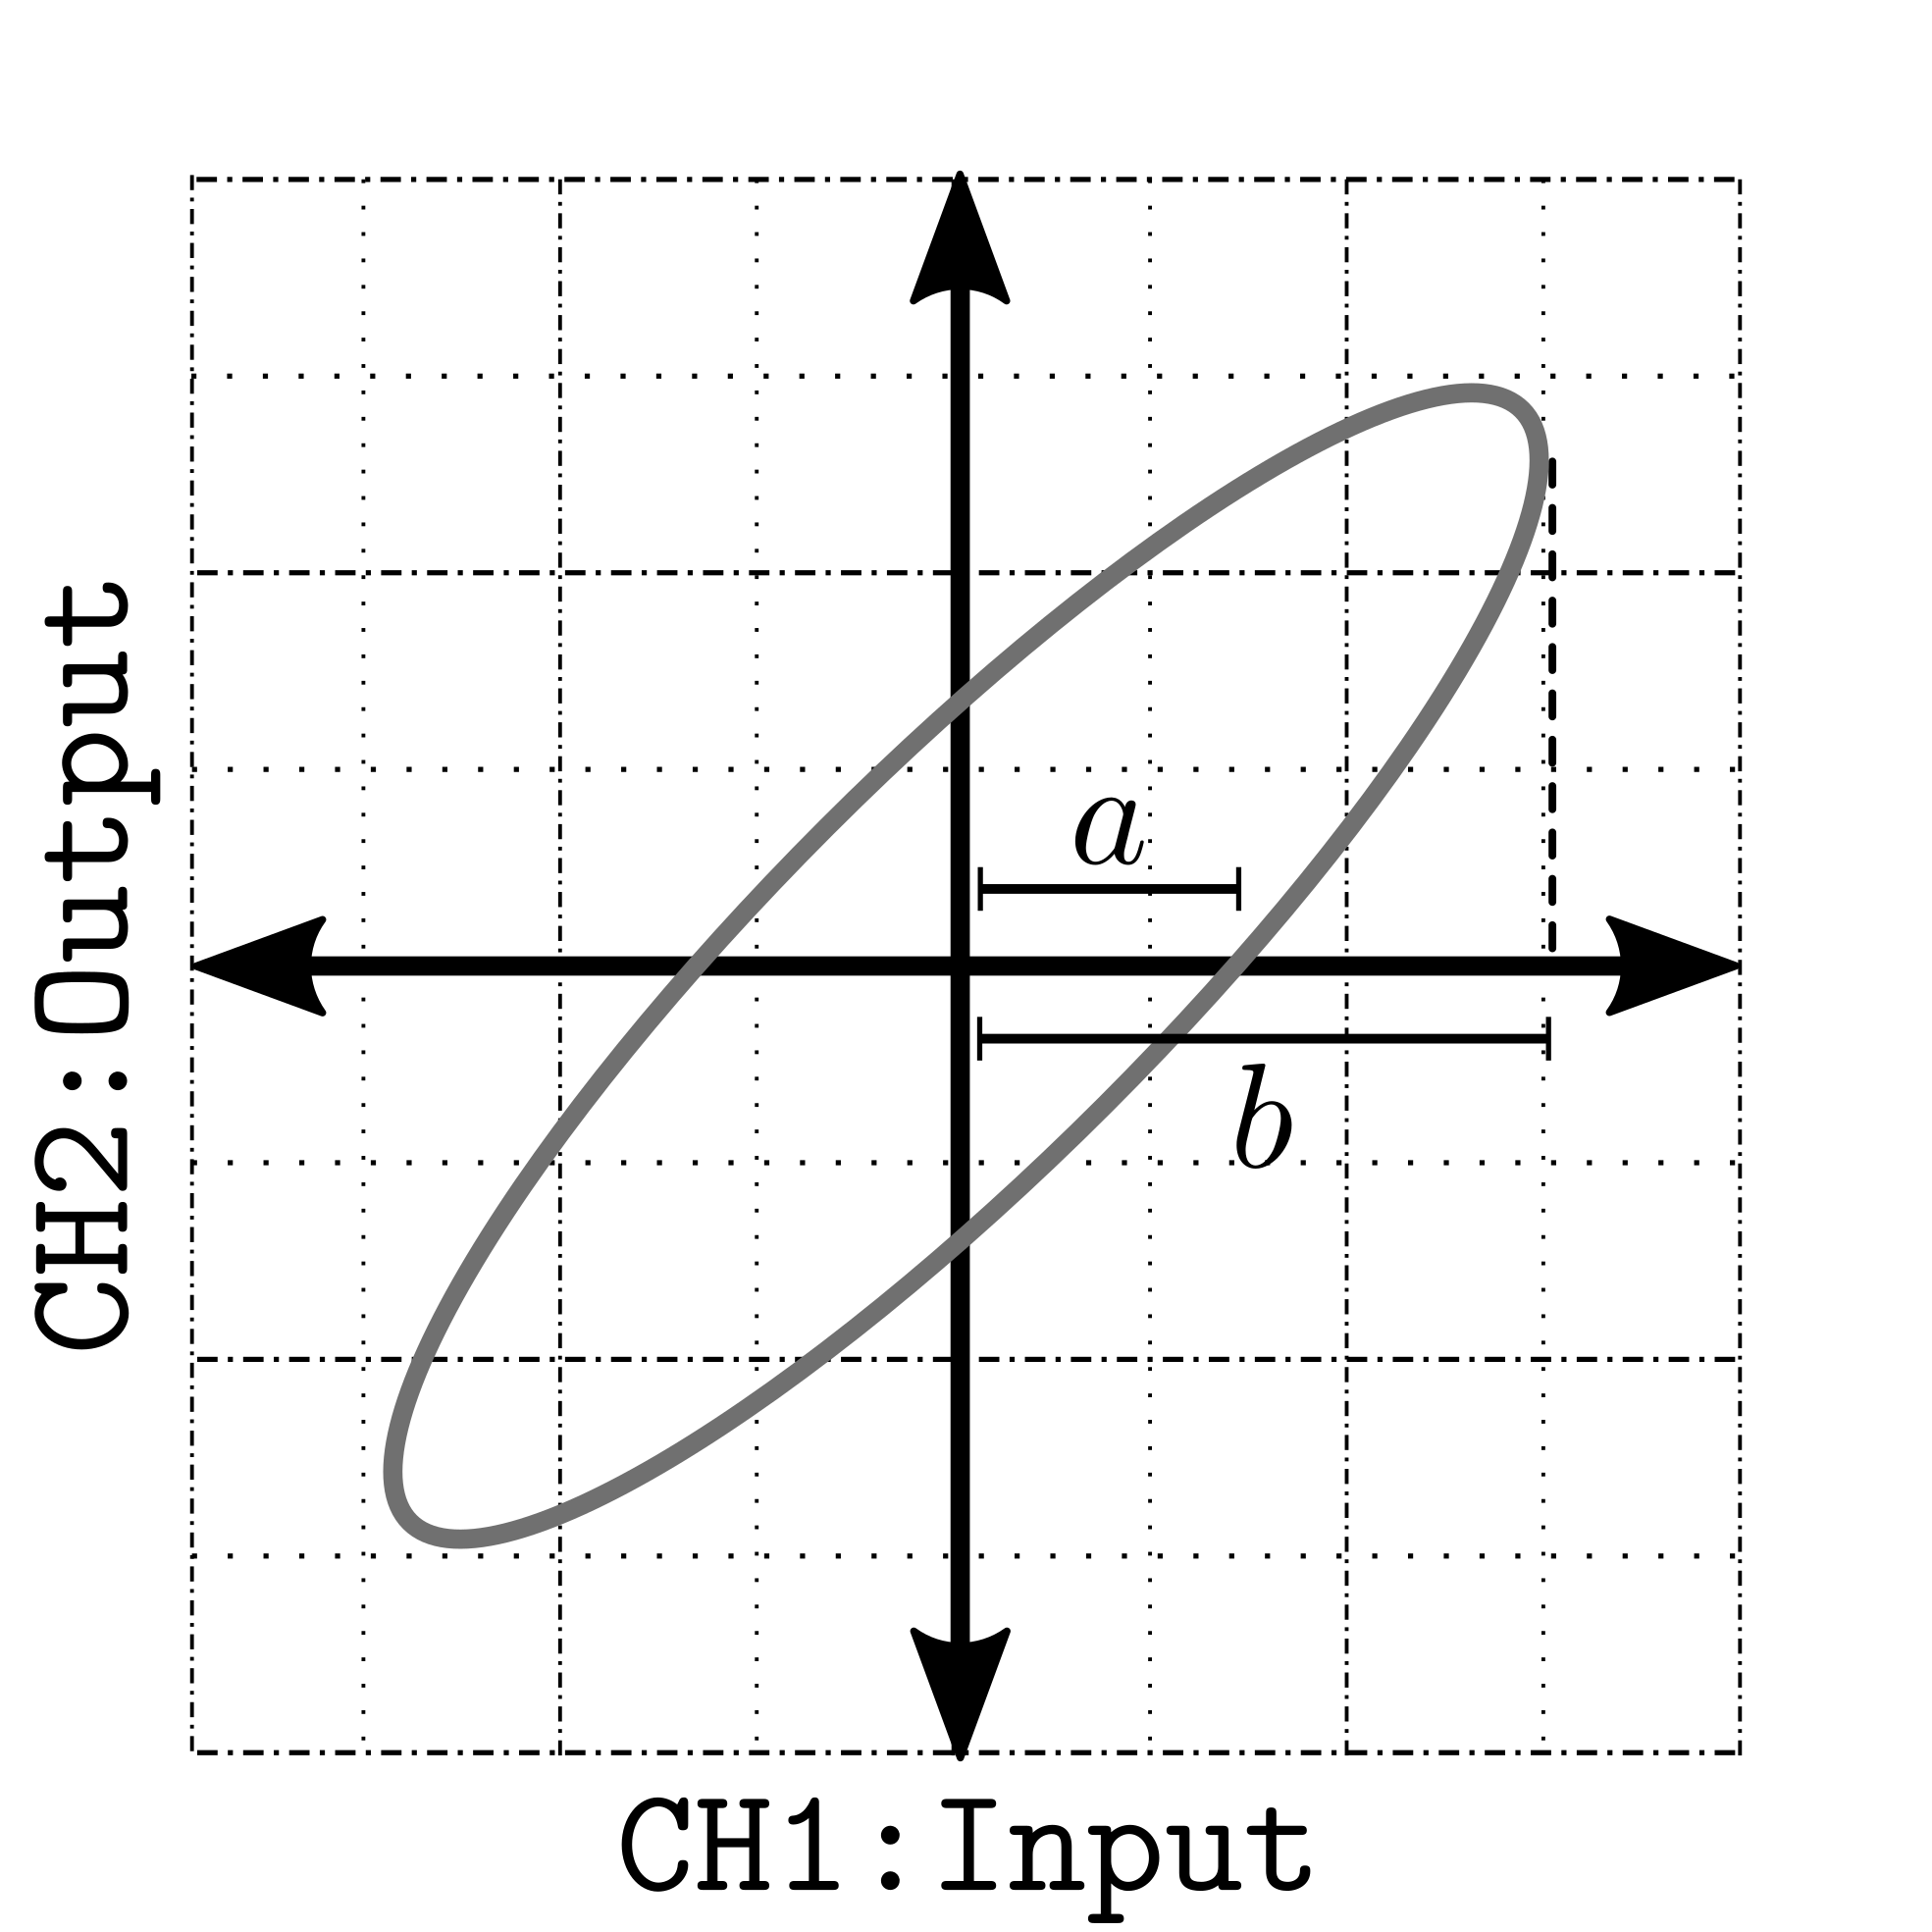
\includegraphics[width=0.4\textwidth]{figs/electronics-circuits/lissajous.png}
    \caption{A Lissajous figure. The input voltage is sent across one of the channels of an oscilloscope, and the voltage across the resistor is sent across the other channel. In the \texttt{XY} mode of the oscilloscope, an ellipse is obtained. $a$ is the positive value of $x$ where $y=0$, and $b$ is the maximum value of $x$ that the ellipse can have. Using $a$ and $b$, the phase difference between the signals can be measured. }
    \label{fig:lissajous}
\end{figure}

\begin{question}
    \textbf{Question:} Consider two orthogonal sinusoids with a frequency $\omega$ and phase difference $\varphi$:
    \begin{equation}
        \begin{aligned}
            x(t) &= A \sin(\omega t + \varphi)\\
            y(t) &= B \sin(\omega t).
        \end{aligned}
    \end{equation}
    Using the above definitions, show that if
    \begin{equation}
        \begin{aligned}
            y(t)&=0 \quad \quad \implies \quad \quad a = A \sin\varphi, \\
            x(t)&=0 \quad \quad \implies \quad \quad b = A.
        \end{aligned}
    \end{equation}

    Use this to show that 
    \begin{equation}
        \varphi = \arcsin\left(\frac{a}{b}\right).
    \end{equation}
\end{question}

\begin{imp}
    \textbf{Important:} In our analysis of the $LCR$ circuit so far, you should notice that unlike the $RC$ circuit, the quantity of interest is the \textsl{current} in the circuit rather than the voltage. Our Digital Oscilloscopes, like most oscilloscopes, measures voltage, and not current. In order to get around this, we measure instead the voltage across the resistor $R$, since $V_R = I R$, and the current in the circuit is simply $I = V_R/R$. Thus, in both the series $LCR$ and ``tank'' circuits described above, the resistor also plays the role of a \textsl{load}.
\end{imp}



\section*{Experimental Setup}

\subsection*{Apparatus}

\begin{enumerate}[label=\arabic*)]
\itemsep0em
\item An assorted set of resistors, capacitors, and inductors
\item A breadboard in which to attach them
\item A function generator
\item A Digital Storage Oscilloscope (DSO)
\item BNC cables
\item A BNC T-connector

\vspace{\parskip}
\begin{imp}
\textbf{Note:}
\begin{itemize}
    \item The output on the screen of the oscilloscope can be saved to a pen-drive. This will be particularly useful if you want to save the input and output waveforms in the case of the integrator and differentiator circuits, for example.
    \item The BNC T-connector can be used to split the signal generated by the function generator into two arms. One arm can be used as the input to the circuit, while the other can be displayed on the oscilloscope. This way, both the input signal and the output signals can be observed on different channels simultaneously.
    \item In all of our analysis so far, we have used \textsl{angular} frequency $\omega$. However, the frequencies produced by the function generator and detected by the DSO are \textsl{linear} frequencies $f$. The relationship between the two is simply
    \begin{equation}
        \omega = 2 \pi f.
    \end{equation}
\end{itemize}
\end{imp}

\end{enumerate}

\subsection*{Precautions}

\begin{itemize}
\item Check the value of each of the component that you will be using \textsl{before} making the circuit, and calculate all the relevant frequencies ($\omega_c$, $\omega_0$) theoretically to make sure they lie in a reasonable range.
\item At both the cutoff and resonant frequencies, the frequency response of our circuits varies very slowly. Consequently, you should vary the frequency in smaller intervals near these regions, so that the behaviour can be seen clearly.
\item Keep the amplitude of the input signal fixed while changing the frequency.
\item Handle the DSO carefully as it is an expensive piece of equipment.
\end{itemize}


\section*{Procedure}

\subsection*{Part A}

In this part of the experiment, you will be studying the $RC$ circuit in the time-domain, and seeing how it can be used as an integrator and a differentiator. 

\begin{enumerate}
    \item Connect the resistor and the capacitor in series as shown in Figure~(\ref{fig:rc-lp}) measure the voltage across the resistor $V_R$.
    \item Connect the function generator to the input of the circuit and the DSO across the output.
    \begin{imp}
        \textbf{Note:} In every case, the voltage has to be taken \textsl{with respect to the ground}, as shown in Figure~(\ref{fig:rc-lp}). This could require some moving about of the components in your circuit.
    \end{imp}

    You can split the input using the BNC T-connector and display both $V_\text{in}$ and $V_\text{out}$ on the oscilloscope.
    \item Feed in a square-wave into the circuit, and observe the output voltage. Show that in the appropriate regime, the output voltage is the integral of the input voltage.

    \item Now repeat the same process for the circuit shown in Figure~(\ref{fig:rc-hp}), and show that in this case, the output voltage is the \textsl{derivative} of the input voltage.

    \item Store these output waveforms and include them in your final report.
\end{enumerate}


\subsection*{Part B}

Using the same two configurations as in \textbf{Part A}, you will now study the $RC$ circuit in the frequency-domain, and observe its frequency response.

\begin{enumerate}
    \item Feed a sinusoidal signal into the $RC$ circuit in the low-pass configuration. Choose a frequency such that $\omega \ll \omega_c$, the cutoff frequency for the system.
    \item Measure the ratio of the output voltage to the input voltage, and use it to compute the gain in dB.
    \item Slowly vary the frequency from $\omega \ll \omega_c$ to $\omega \gg \omega_c$, computing the gain at every value.
    \item Plot a Bode plot for the low-pass filter, and compare it to Figure~(\ref{fig:RC-bode}).
    \item Repeat the above process for the high-pass filter configuration.
\end{enumerate}

\subsection*{Part C}

We will now study the frequency response of the $LCR$ circuit in both the series and the parallel ``tank'' configuration.

\begin{enumerate}
    \item Connect the inductor, resistor, and capacitor as shown in Figure~(\ref{fig:lcr-series}), and measure the voltage across the resistor $V_R$. Remember that this is a measure of the \textsl{current} in the circuit.
    \item Feed a sinusoidal signal of frequency $\omega \ll \omega_0$, the natural frequency of the oscillator. Keep the amplitude of the input waveform fixed and vary its frequency, measuring the gain at every step.
    \item Plot a Bode plot for the frequency response of the series $LCR$ circuit.
    
    \item Similarly, make the connections for tank circuit, as shown in Figure~(\ref{fig:lcr-parallel}), and plot a similar Bode plot for its frequency response.
    \item Show that the frequency response of both the $LCR$ circuits described above appear inverted with respect to each other.
\end{enumerate}